% 独自のコマンド

% ■ アブストラクト
%  \begin{jabstract} 〜 \end{jabstract}  :日本語のアブストラクト
%  \begin{eabstract} 〜 \end{eabstract}  :英語のアブストラクト

% ■ 謝辞
%  \begin{acknowledgment} 〜 \end{acknowledgment}

\newif\ifjapanese

\japanesetrue  % 論文全体を日本語で書く(英語で書くならコメントアウト)

\ifjapanese
  \documentclass[a4j,twoside,openright,11pt]{jreport} % 両面印刷の場合。余白を綴じ側に作って右起こし。
  %\documentclass[a4j,11pt]{jreport}                  % 片面印刷の場合。
  \renewcommand{\bibname}{参考文献}
  \newcommand{\acknowledgmentname}{謝辞}
\else
  \documentclass[a4paper,11pt]{report}
  \newcommand{\acknowledgmentname}{Acknowledgment}
\fi
\usepackage[dvipdfmx]{graphicx}
\usepackage{thesis}
\usepackage{ascmac}
\usepackage{graphicx}
\usepackage{multirow}
\usepackage{url}
\usepackage{latexsym}
\usepackage{here}
\usepackage{listings,jlisting}

\lstset{%
  language={C},
  basicstyle={\small\ttfamily\footnotesize},%
  breaklines=true,%
  identifierstyle={\small},%
  commentstyle={\small\itshape},%
  keywordstyle={\small\bfseries},%
  ndkeywordstyle={\small},%
  stringstyle={\small\ttfamily},
  frame={tb},
  breaklines=true,
  columns=[l]{fullflexible},%
  numbers=left,%
  xrightmargin=0zw,%
  xleftmargin=3zw,%
  numberstyle={\scriptsize},%
  stepnumber=1,
  numbersep=1zw,%
  lineskip=-0.5ex%
}
\bibliographystyle{jplain}

\bindermode  % ファイル綴じ用余白設定

% 日本語情報(必要なら)
\jclass  {修士論文}                             % 論文種別
\jtitle  {ハイパー楽譜システムの研究}      % タイトル。改行する場合は\\を入れる
\juniv   {慶應義塾大学大学院}                   % 大学名
\jfaculty{政策・メディア研究科}                 % 学部、学科
\jauthor {佐竹 紘明}                            % 著者
\jhyear  {30}                                   % 平成○年度
\jsyear  {2018}                                 % 西暦○年度
\jkeyword{ユーザーインターフェース、楽譜、ハイパーテキスト、IME、hoge}       % 論文のキーワード
\jproject{インタラクションデザインプロジェクト} % プロジェクト名
\jdate   {2019年1月}

% 英語情報(必要なら)
\eclass  {Master's Thesis}                          % 論文種別
\etitle  {A \LaTeX Template for Master Thesis}      % タイトル。改行する場合は\\を入れる
\euniv   {Keio University}                          % 大学名
\efaculty{Graduate School of Media and Governance}  % 学部、学科
\eauthor {Hiroaki Satake}                                % 著者
\eyear   {2018}                                     % 西暦○年度
\ekeyword{User Interface, Musical Notation, Hypertext, IME, hoge}          % 論文のキーワード
\eproject{Interaction Design Project}               % プロジェクト名
\edate   {January 2019}


\begin{document}

\ifjapanese
  \jmaketitle    % 表紙(日本語)
\else
  \emaketitle    % 表紙(英語)
\fi

t% ■ アブストラクトの出力 ■
%	◆書式:
%		begin{jabstract}〜end{jabstract}	:日本語のアブストラクト
%		begin{eabstract}〜end{eabstract}	:英語のアブストラクト
%		※ 不要ならばコマンドごと消せば出力されない。



% 日本語のアブストラクト
\begin{jabstract}

テンプレートの説明を、テンプレート自身を使って説明する。これは @kurokobo による卒業論文のための\LaTeX テンプレートを修士論文用に改造し、さらにUTF-8化やMakefile等の添付をしたものである。

この部分には一般には論文のアブストラクトを書く。日本語のアブストラクトを書きたいなら、\verb|\begin{jabstract}| と \verb|\end{jabstract}| の間に文章を書けば、今のこのページのように体裁が勝手に整って出力される。英語のアブストラクトは \verb|\begin{eabstract}| と \verb|\end{eabstract}| の間に書けば、次ページのような体裁で出力される。

両方を書けば、日本語と英語の両方のアブストラクトが並んで出力される(この文書はサンブルなので両方書いてある)。ページ順序は、コマンドを書いた順序の通り。どちらか一方のみを出力したい場合は、不要な方をコマンド自体を含め削除する。

このあたりの詳細もあとで書く。基本的には、{\tt main.tex}を上から順にいじっていけばできるはず。

\end{jabstract}



% 英語のアブストラクト
\begin{eabstract}

Eigo ga dekinai node Roma-ji de soreppoi hunniki wo daseruto iina.

Murippoi desu ne.

Write down your abstract here. Write down your abstract here. Write down your abstract here. Write down your abstract here. Write down your abstract here. Write down your abstract here.

 Write down your abstract here. Write down your abstract here. Write down your abstract here. Write down your abstract here. Write down your abstract here. Write down your abstract here. Write down your abstract here. Write down your abstract here. Write down your abstract here. Write down your abstract here. Write down your abstract here. Write down your abstract here.
 
Write down your abstract here. Write down your abstract here.

\end{eabstract}
  % アブストラクト。要独自コマンド、include先参照のこと

\tableofcontents  % 目次
\listoffigures    % 表目次
\listoftables    % 図目次

\pagenumbering{arabic}

\chapter{序論}
\label{chap:introduction}

本章では本研究の動機と目的、および本論文の構成について述べる。

\newpage

\section{研究の動機}

楽譜は17世紀ごろに五線譜による近代記譜法のフォーマットが確立してからほとんど形態が変わっておらず、今日においても国際的かつ普遍的な記法として広く利用されている。
これは楽譜が優れた表現力を持ち、様々な音楽を記録するのに適していることにほかならない。
しかし当初から印刷を前提としたフォーマットであったため、以下のような問題も存在する。

\begin{itemize}
    \item 簡単に編集できない
    \item メモなどの情報を自在に書けない
    \item 参照や管理が面倒
\end{itemize}

また計算機が普及した現在では楽譜を快適に閲覧したり、美しい楽譜を作成できるソフトウェアも広く利用されているが、PDFのように内容の変更が不可能な形式で楽譜を管理することが一般的であり、紙の楽譜と本質的な特徴は変わっていない。
一方、楽譜と同様に紙の上に記録されていたテキストは計算機の登場によって以下のような進化を遂げた。

\begin{itemize}
    \item コピー/ペースト/Undo/Redoといったテキスト編集支援機能が手軽な編集を可能にした
    \item IMEといったテキスト入力支援機能が手軽な入力を可能にした
    \item ハイパーテキストがマルチメディアを活用した分かりやすいドキュメントの作成や、ハイパーリンクを可能にした
    \item Webが様々なドキュメントへの素早いアクセスを可能にした
    \item Wikiのようなコラボレーションツールが複数人による共同編集を可能にした
\end{itemize}

これらの進化によって、紙というメディアの特性上ドキュメントが物理的に独立していて内容の変更も難しいという性質が消えてしまった。
かつては楽譜と同じ問題を抱えていたが、計算機によって新しい便利な使い方が発明され、広く普及したのである。
楽譜はフォーマットや使い方が数百年変わっていないので、計算機によって進化する余地はまだまだ存在すると考えられる。

\section{研究の目的}
本研究では、上記のような楽譜が持つ問題点を解決し、これまでの楽譜の在り方にとらわれない次世代の楽譜システム「ハイパー楽譜システム」の構築を目的とする。
ハイパーテキストやWikiの手法を取り入れることで、従来の楽譜システムでは実現できなかった快適な楽譜編集・利用環境を実現する。

\section{本論文の構成}

本論文は以下の9章で構成される。

第2章では、本研究の背景をより詳細に分析し、楽譜の問題点を整理する。

第3章では、本論文で提案するシステムの基本構成と使い方について述べる。

第4章では、本論文で提案するシステムの詳細な実装について述べる。

第5章では、本論文で提案するシステムで利用できる楽譜IMEを提案する。

第6章では、本論文で提案するシステムによって実現可能な応用例について述べる。

第7章では、関連する研究を紹介し、それらの特徴や本研究との関連を述べる。

第8章では、筆者による運用経験やユーザーからのフィードバックをまとめ、本論文で提案するシステムの有効性と問題点について述べる。

最後に、第9章で本論文のまとめと結論を述べる。
  % 本文1
\chapter{研究背景}
\label{chap:haikei}

本章では楽譜の問題点と、楽譜を扱う既存システムの現状を整理する。

\newpage

\section{楽譜}

楽譜は楽曲を記号や文字によって書き表したものである。
一般に五線譜のことを指すことが多いが、ギター演奏用に利用されるタブ譜や日本固有の三味線譜など、用途やジャンル、地域によって様々な種類の楽譜が存在する。
西洋音楽をルーツに持つ五線譜は国際的かつ普遍的なものとして認められており、現在は様々な音楽を記録するために広く利用されている。

\section{楽譜の歴史}

本節では今日利用されている楽譜が生まれるまでの進化の歴史を概観する\cite{Minagawa}。

\subsection{ネウマ譜}
ネウマ譜(図\ref{neume})は旋律の上行下行の動きをネウマと呼ばれる線状の記号で表示する記譜法で、9世紀頃から中世キリスト教会の典礼音楽であったグレゴリオ聖歌の記譜のために用いられはじめた。
10-11世紀ごろからは横線(譜線)を添えて、音程関係を明確にする試みが行われた。
譜線が添えられている限りは音高が明確だが、リズムの表示はあいまいである。

\begin{figure}[H]
    \centering
    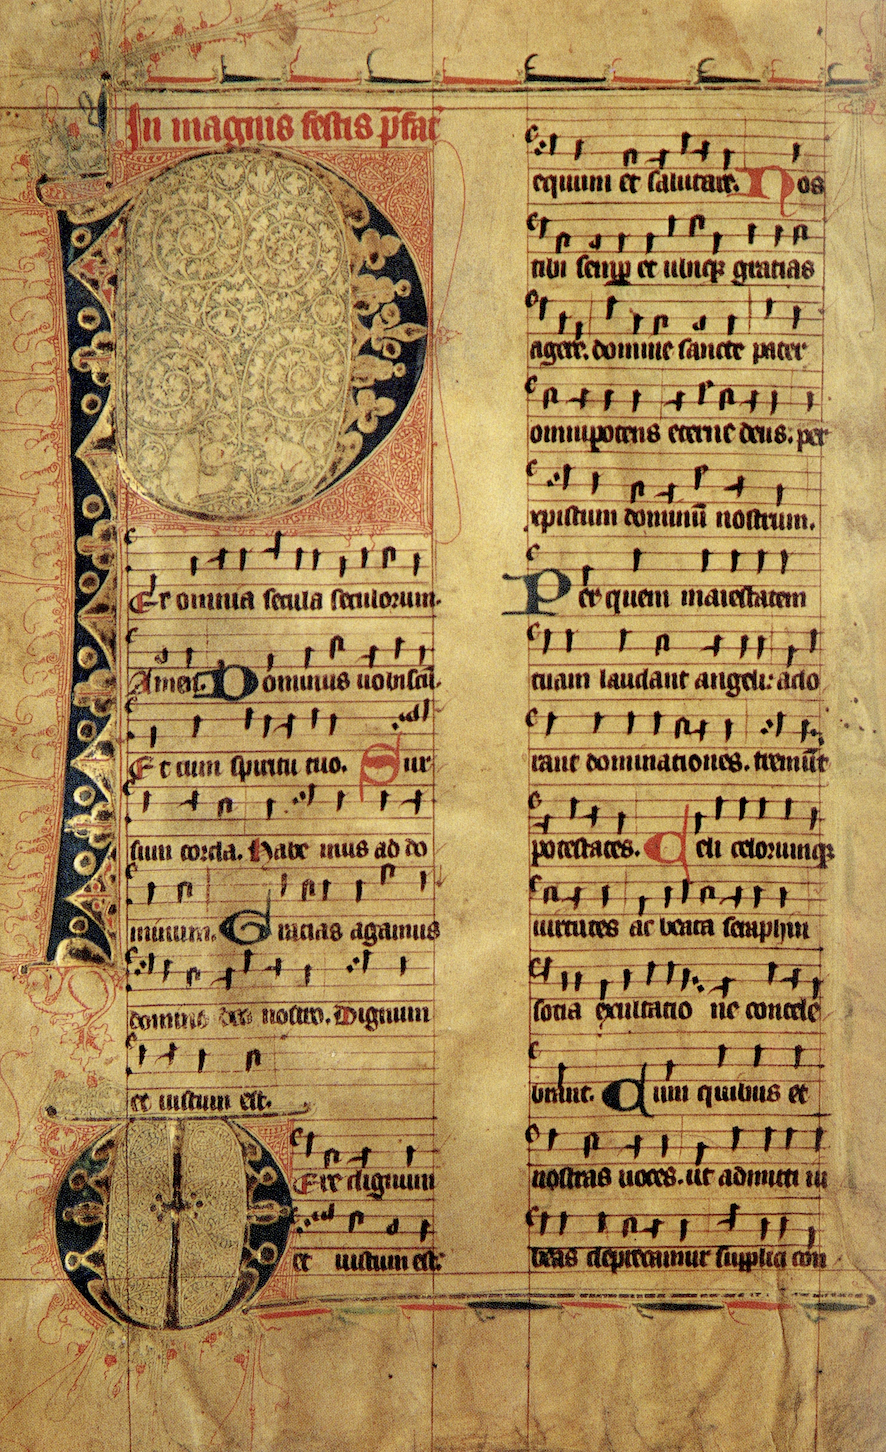
\includegraphics[width=7cm]{images/neume.png}
    \caption{ネウマ譜の例}
    \label{neume}
\end{figure}

\subsection{定量譜}
複数の奏者がそれぞれ異なった声部を同時に演奏する多声音楽が生まれると、リズム表示があいまいな従来のネウマ譜では不十分となった。
13世紀後半になると、音の長短を音符の形状で区別する定量譜(図\ref{teiryo})が利用されるようになった。

\begin{figure}[H]
    \centering
    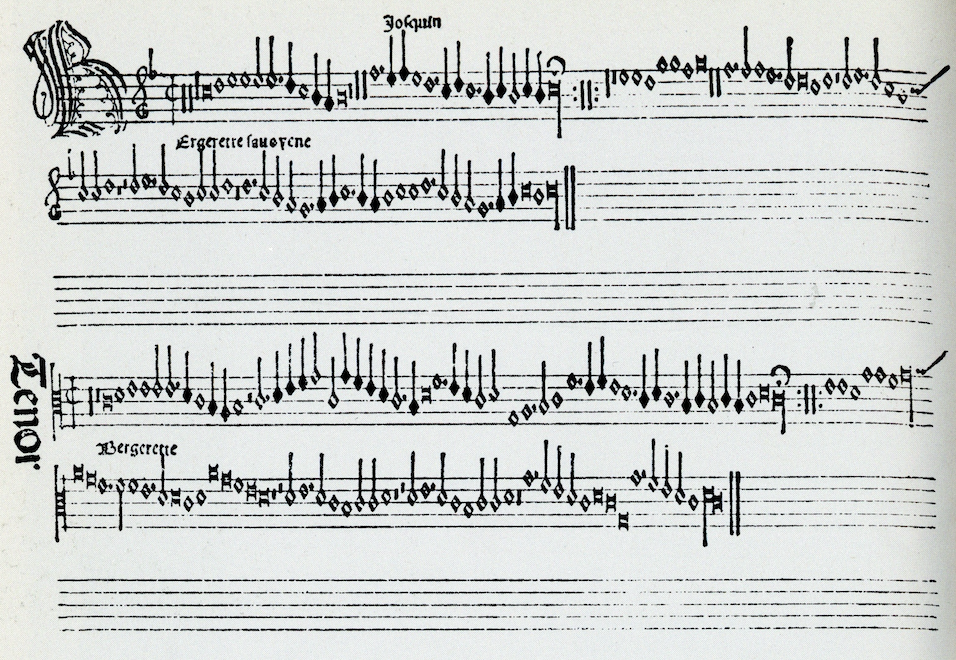
\includegraphics[width=9cm]{images/teiryo.png}
    \caption{定量譜の例}
    \label{teiryo}
\end{figure}

\subsection{奏法譜}
15世紀ごろからは特定の楽器の演奏法を具体的に表示する奏法譜(図\ref{tab})も広く利用された。
楽器ごとに固有の奏法譜をもち、現代でも「タブ譜」としてギター演奏に利用されている。

\begin{figure}[H]
    \centering
    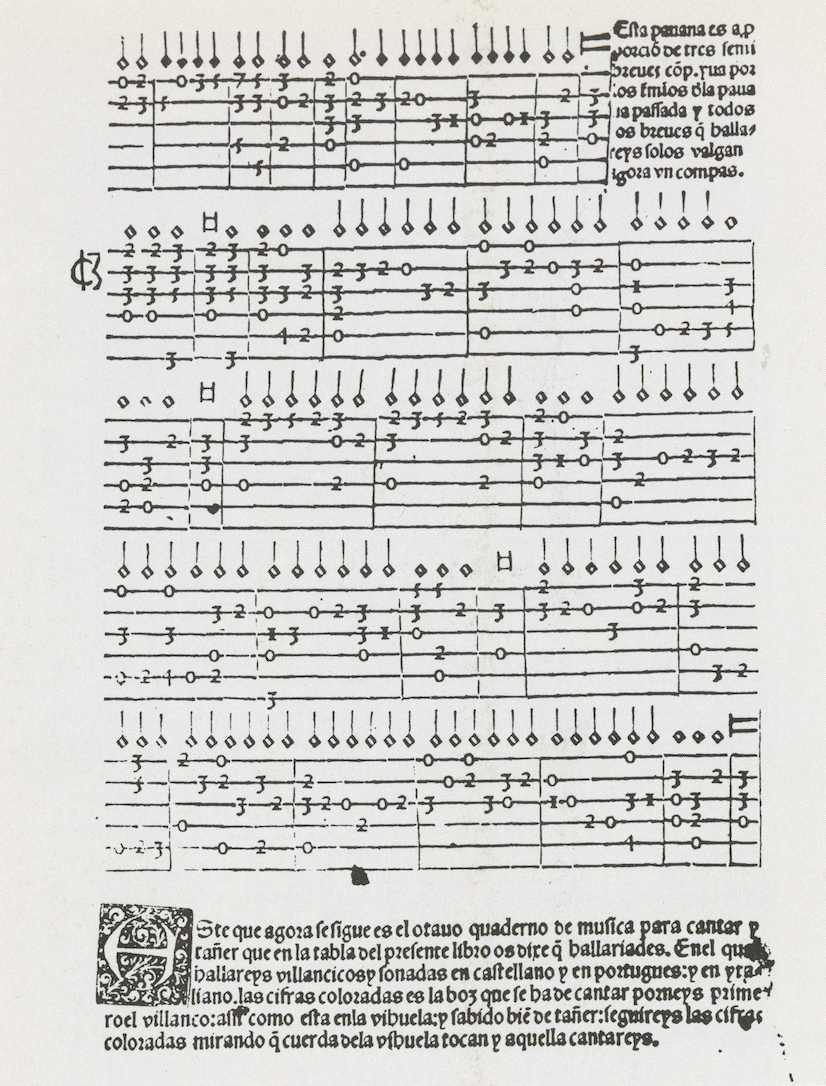
\includegraphics[width=6cm]{images/tab.png}
    \caption{奏法譜の例}
    \label{tab}
\end{figure}

\subsection{近代譜}
17世紀初頭から現在までに世界で最も普及している楽譜の形態(図\ref{kindai})で、鍵盤楽器用の奏法譜をルーツに持つ。
\begin{itemize}
    \item 五線による音高表示
    \item 音符の「はた」によるリズム表示
    \item 小節線の使用
\end{itemize}といった特徴がある。

\begin{figure}[H]
    \centering
    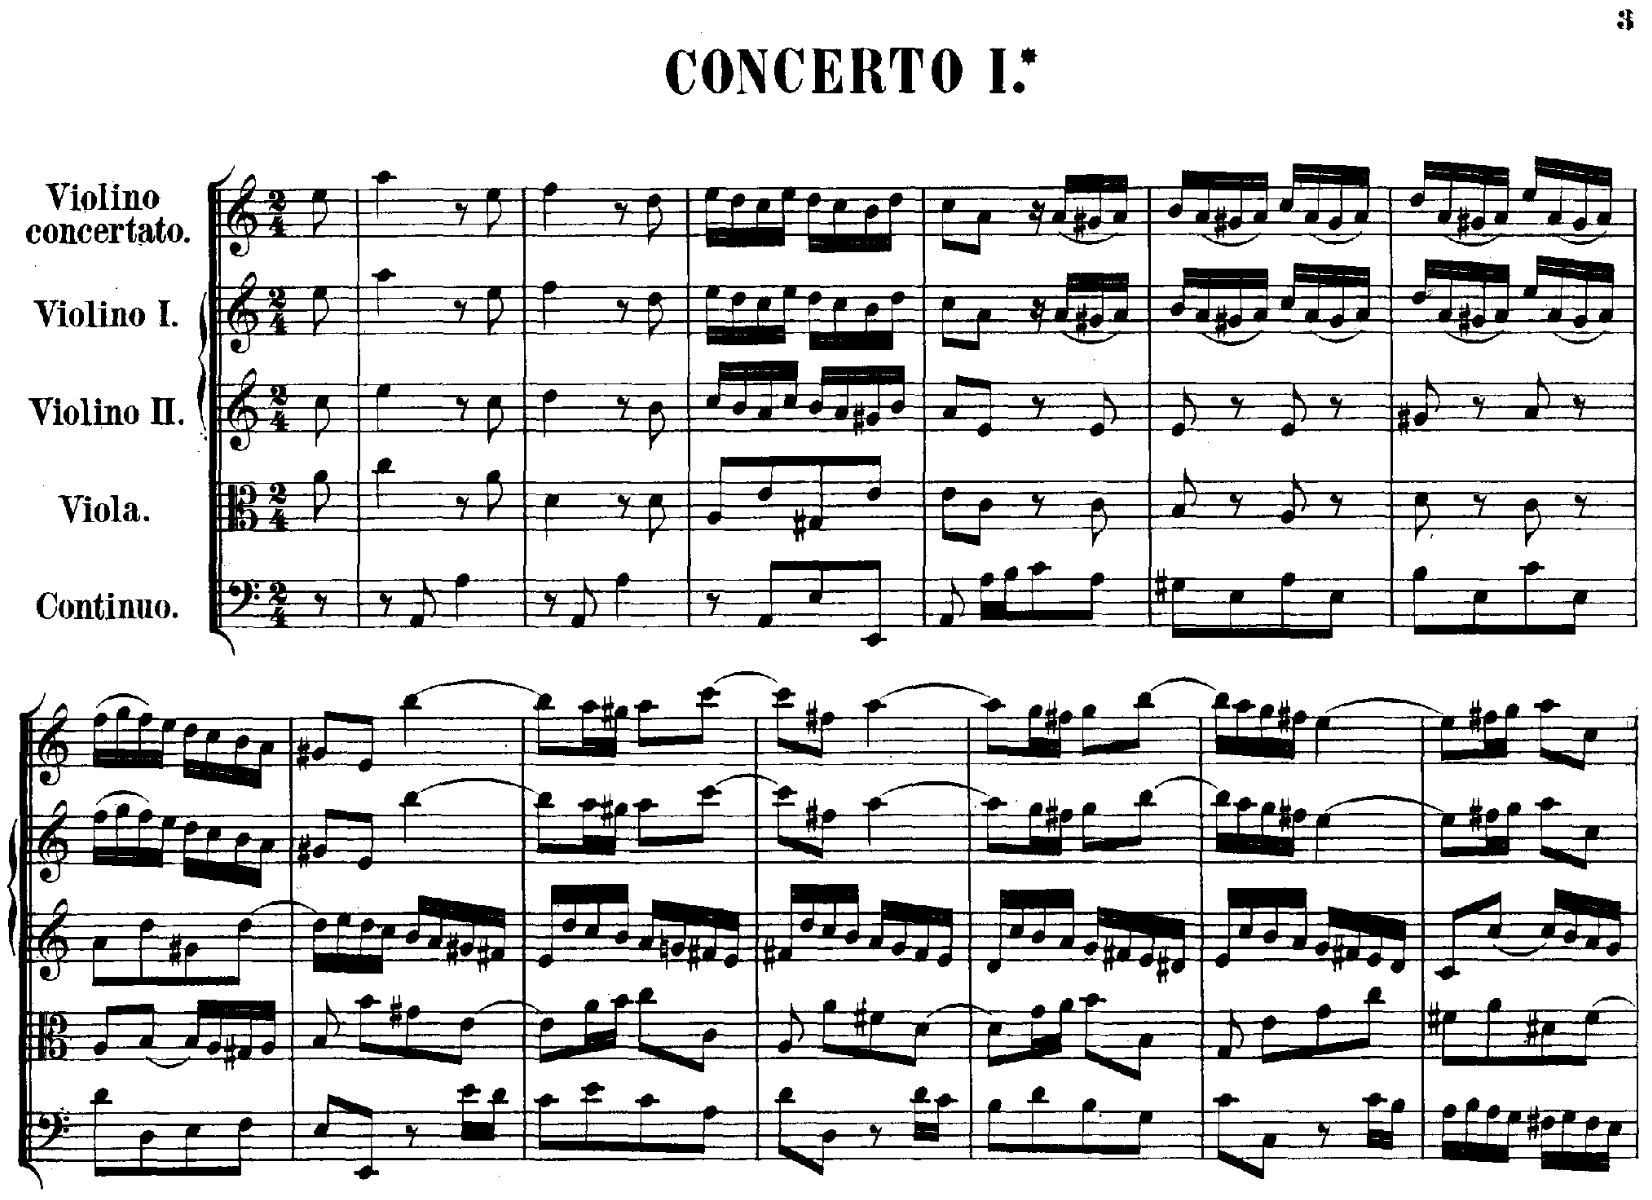
\includegraphics[width=9cm]{images/kindai.png}
    \caption{近代譜の例}
    \label{kindai}
\end{figure}

\subsection{現代音楽}
五線譜は鍵盤楽器をベースにした西洋音楽に最適化された記譜法のため、半音以下の繊細な音程のゆれや微妙なニュアンスを表現できないという制約がある。
現代の作曲家たちはそれぞれ独自の方法で克服しようと試みている(図\ref{kondo})。

\begin{figure}[H]
    \centering
    \includegraphics[width=9cm]{images/kondo.png}
    \caption{現代音楽譜の例}
    \label{kondo}
\end{figure}

\section{テキストの進化}
楽譜同様に紙の上で利用されていたテキストの進化にも注目する。
計算機が普及する以前のテキストは印刷物であるという制約から以下のような問題が存在した。
\begin{itemize}
    \item 簡単に編集できない
    \item せいぜい挿絵や写真程度の情報しか一緒に記録できない
    \item ドキュメントが複数存在するとき参照や管理が面倒
\end{itemize}

しかし現在では計算機の進化によりこれらの問題は完全に解決されている。
\begin{itemize}
    \item 手軽な編集\\
    計算機上でテキストを扱えるようになり、コピー/ペースト/Undo/Redoといったテキスト編集支援機能を搭載した各種エディタによって手軽な編集が可能になった。
    また印刷レイアウトを簡単に構成できるワープロソフトによって、美しいレイアウトの文章を簡単に作れるようになった。
    \item 手軽な入力\\
    日本語入力などの文字変換をサポートするシステム(IME)などによって手軽な入力が可能になった。
    \item マルチメディアの活用\\
    画像/音声/動画といったマルチメディアを自在に埋め込むことができるハイパーテキスト(図\ref{hy})によって、情報量の多いドキュメントの作成が可能になった。
    \item ハイパーリンク\\
    ハイパーテキストでは文章間リンクを示すハイパーリンク機能が利用でき、関連情報への素早いアクセスが可能になった。
    \item Web\\
    インターネット技術の進化とWebの普及によって、世界中に存在する様々なドキュメントへ瞬時にアクセスすることが可能になった。
    \item 共同編集\\
    Wikiのようなコラボレーションツールによって、場所や人数に制約を受けない共同編集が可能になった。
\end{itemize}


\begin{figure}[H]
    \centering
    \fbox{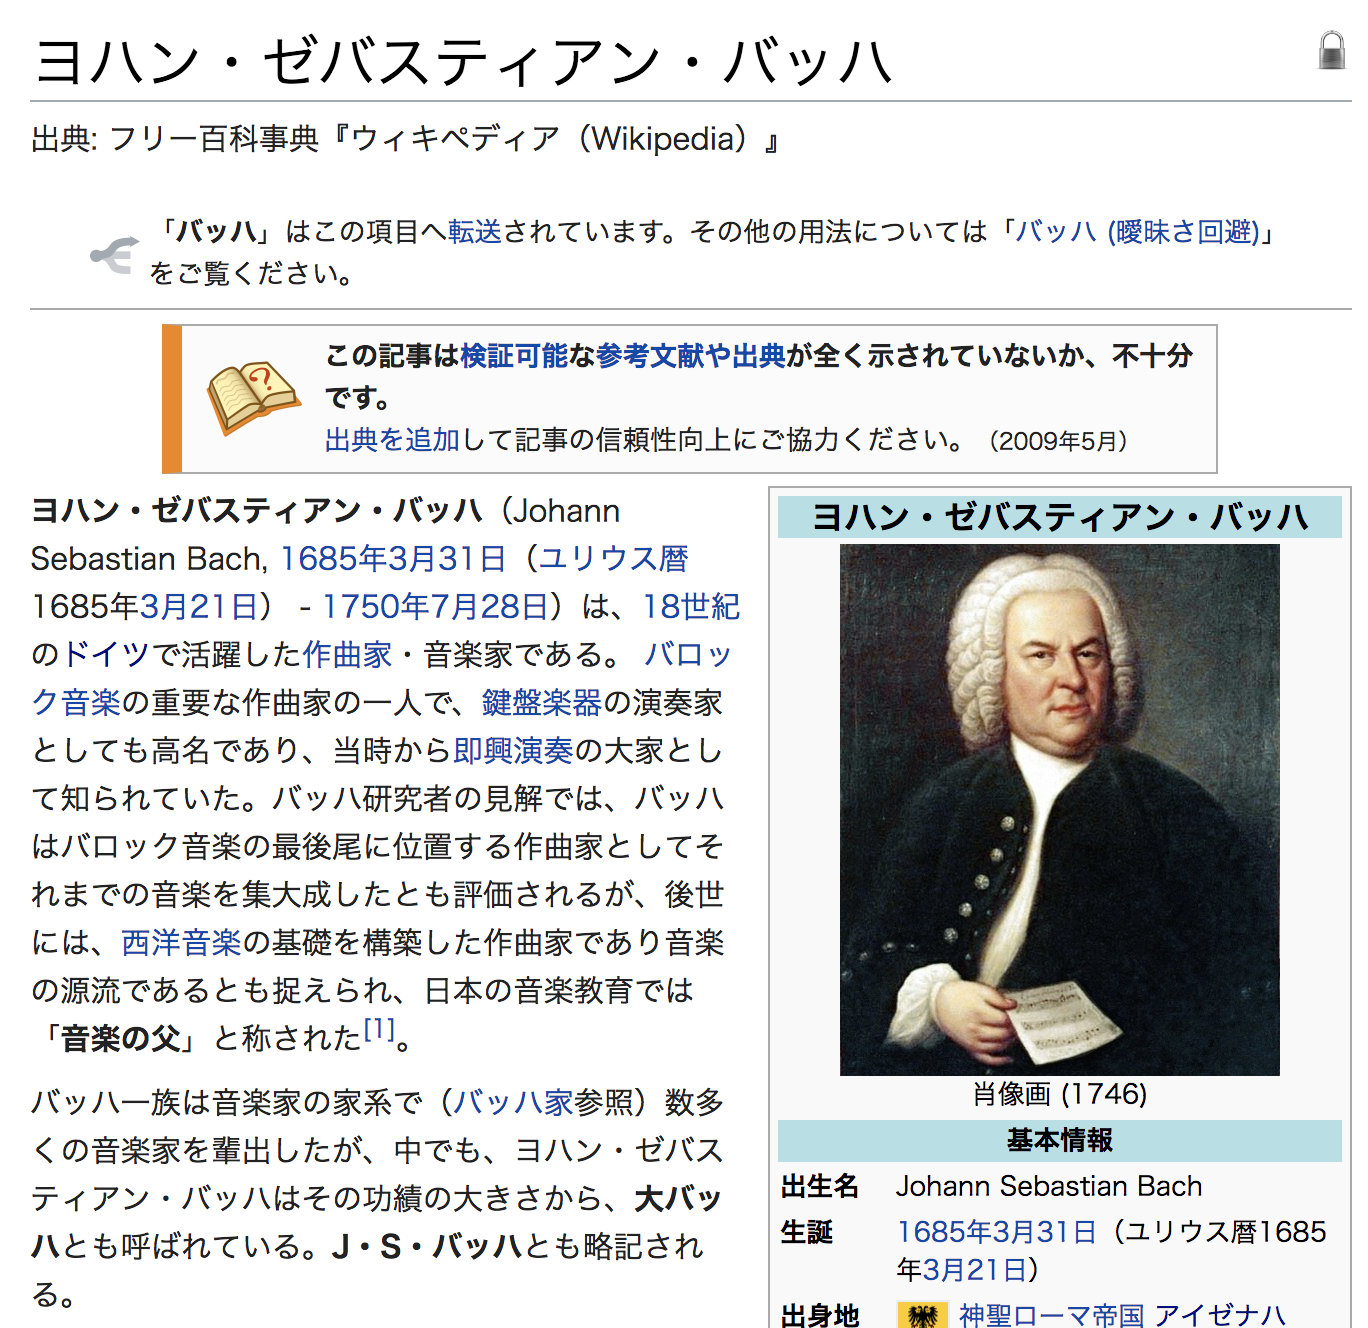
\includegraphics[width=9cm]{images/wikipedia.png}}
    \caption{ハイパーテキストの例}
    \label{hy}
\end{figure}

\section{楽譜の問題点}
\label{mondai}
一方、楽譜の性質は計算機の普及後も印刷物の時代から進化しておらず、以下のような問題が存在する。
\begin{enumerate}
    \item 簡単に編集できない\\
    現在流通している楽譜は紙やPDF形式での配布が一般的であり、内容の変更は前提とされていない。
    また自分で楽譜を書く場合は楽譜作成ソフトを利用できるが、印刷を前提としたレイアウトでの編集を強制されるため、一部だけアレンジしたい・1フレーズだけメモしたいといった用途には向いていない。
    \item メモなどの情報を自在に書けない\\
    楽譜を利用する際には、
    \begin{itemize}
        \item 演奏時に気付いたこと
        \item 演奏時に気をつけるべきこと
        \item 先生に習ったこと
    \end{itemize}などのメモを書き込みながら使うのが一般的である(図\ref{memo})。
    メモ書きできるのは余白スペースだけであり、楽譜自体に編集を加えてレイアウトを変更したり、音声や動画といった文字以外の情報を埋め込むことも不可能なので、記述できる内容は必然的に限られる。
    \item 参照や管理が面倒\\
    紙やPDFはそれぞれが独立しているため、手元の楽譜が増えると管理に苦労する。
    ファイル名でしか楽譜の内容を判断できないため、作曲者別にフォルダを分割するといったファイルの階層的な整理が必要である。
    また楽器構成や年代といった別の側面から参照したい場合には別途索引を用意しなければならない。
\end{enumerate}

\begin{figure}[H]
    \centering
    \fbox{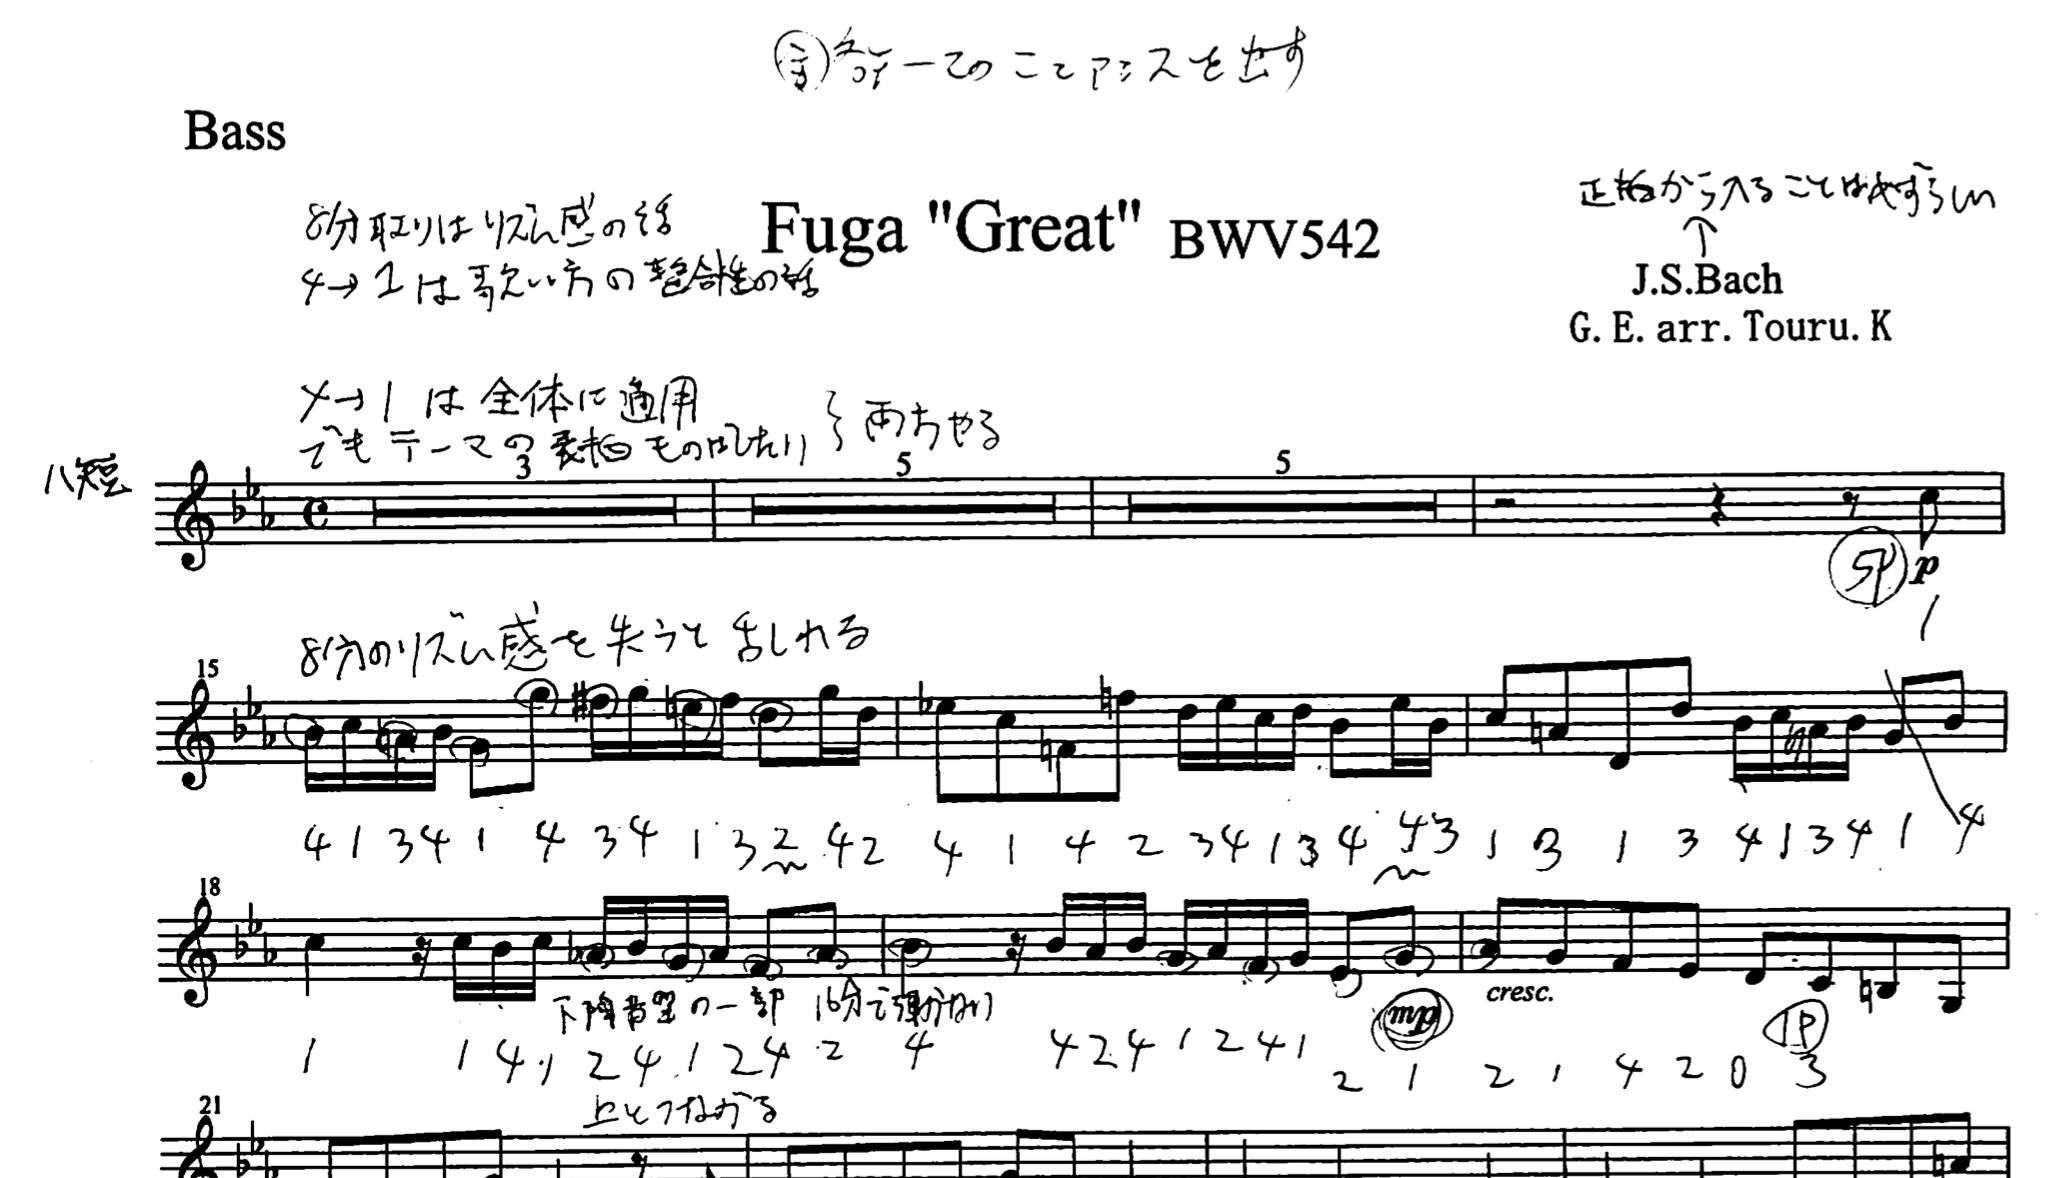
\includegraphics[width=10cm]{images/fuga.png}}
    \caption{楽譜上のメモの例}
    \label{memo}
\end{figure}

\section{既存の楽譜システム}
現在広く利用されている楽譜利用システムを解説する。
\subsection{楽譜作成ソフト}
Finale\footnote{\textsf{https://www.finalemusic.jp/}}(図\ref{finale})、Sibelius\footnote{\textsf{http://www.sibelius.jp/}}といった楽譜作成ソフトがデファクトスタンダードとして商用・私用問わず広く利用されている。
スタンプ感覚で音符を入力できるWYSIWYGな編集環境を持ち、以下のような楽譜作成支援機能を利用できる。
\begin{itemize}
    \item 楽譜スキャン・OCR
    \item パート譜自動作成
    \item レイアウトの細かい微調整
\end{itemize}

\begin{figure}[H]
    \centering
    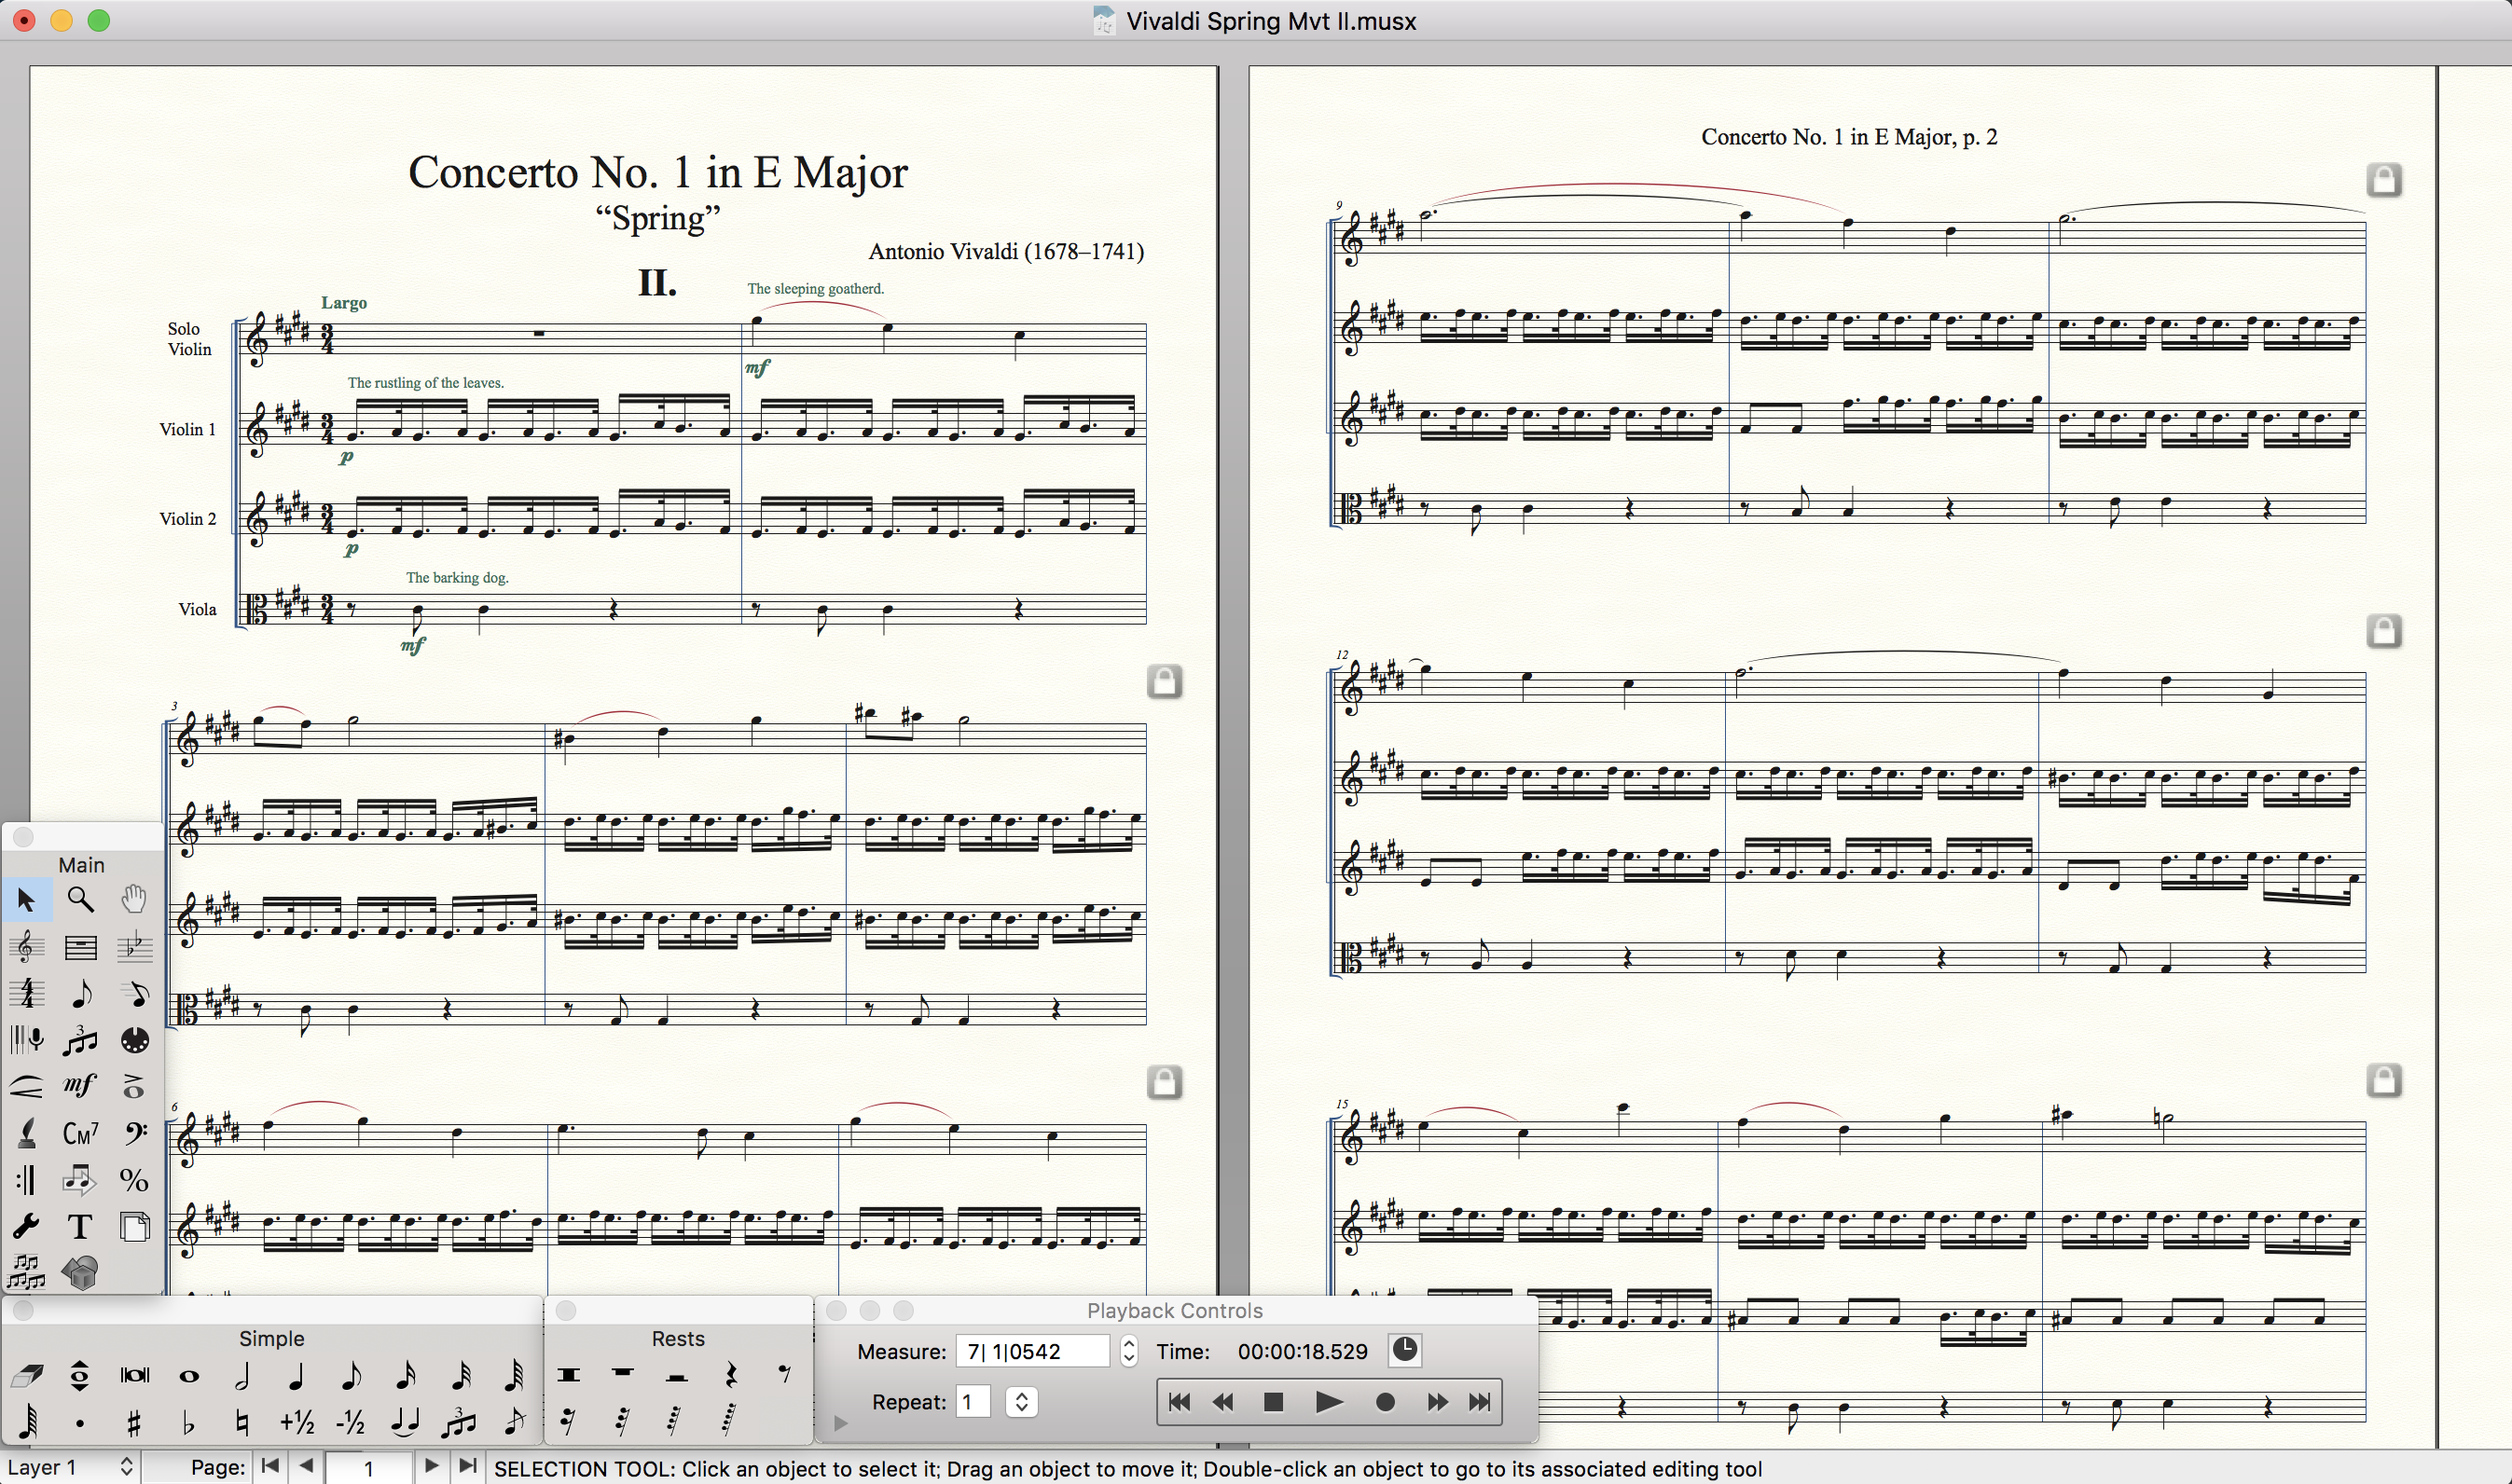
\includegraphics[width=10cm]{images/finale.png}
    \caption{Finaleの画面}
    \label{finale}
\end{figure}

\subsection{楽譜ビューアー}
ほとんどの楽譜はPDFファイルとして配布されるため、閲覧のために標準のPDFビューアーが利用されることが多い。
またPiascore\footnote{\textsf{http://piascore.com/}}(図\ref{pia})を代表とするタブレット端末向けの楽譜に特化したビューアーも広く普及しており、
\begin{itemize}
    \item 楽譜への書き込み
    \item 自動譜めくり
    \item メトロノーム
\end{itemize}といった機能を利用できる。

\begin{figure}[H]
    \centering
    \fbox{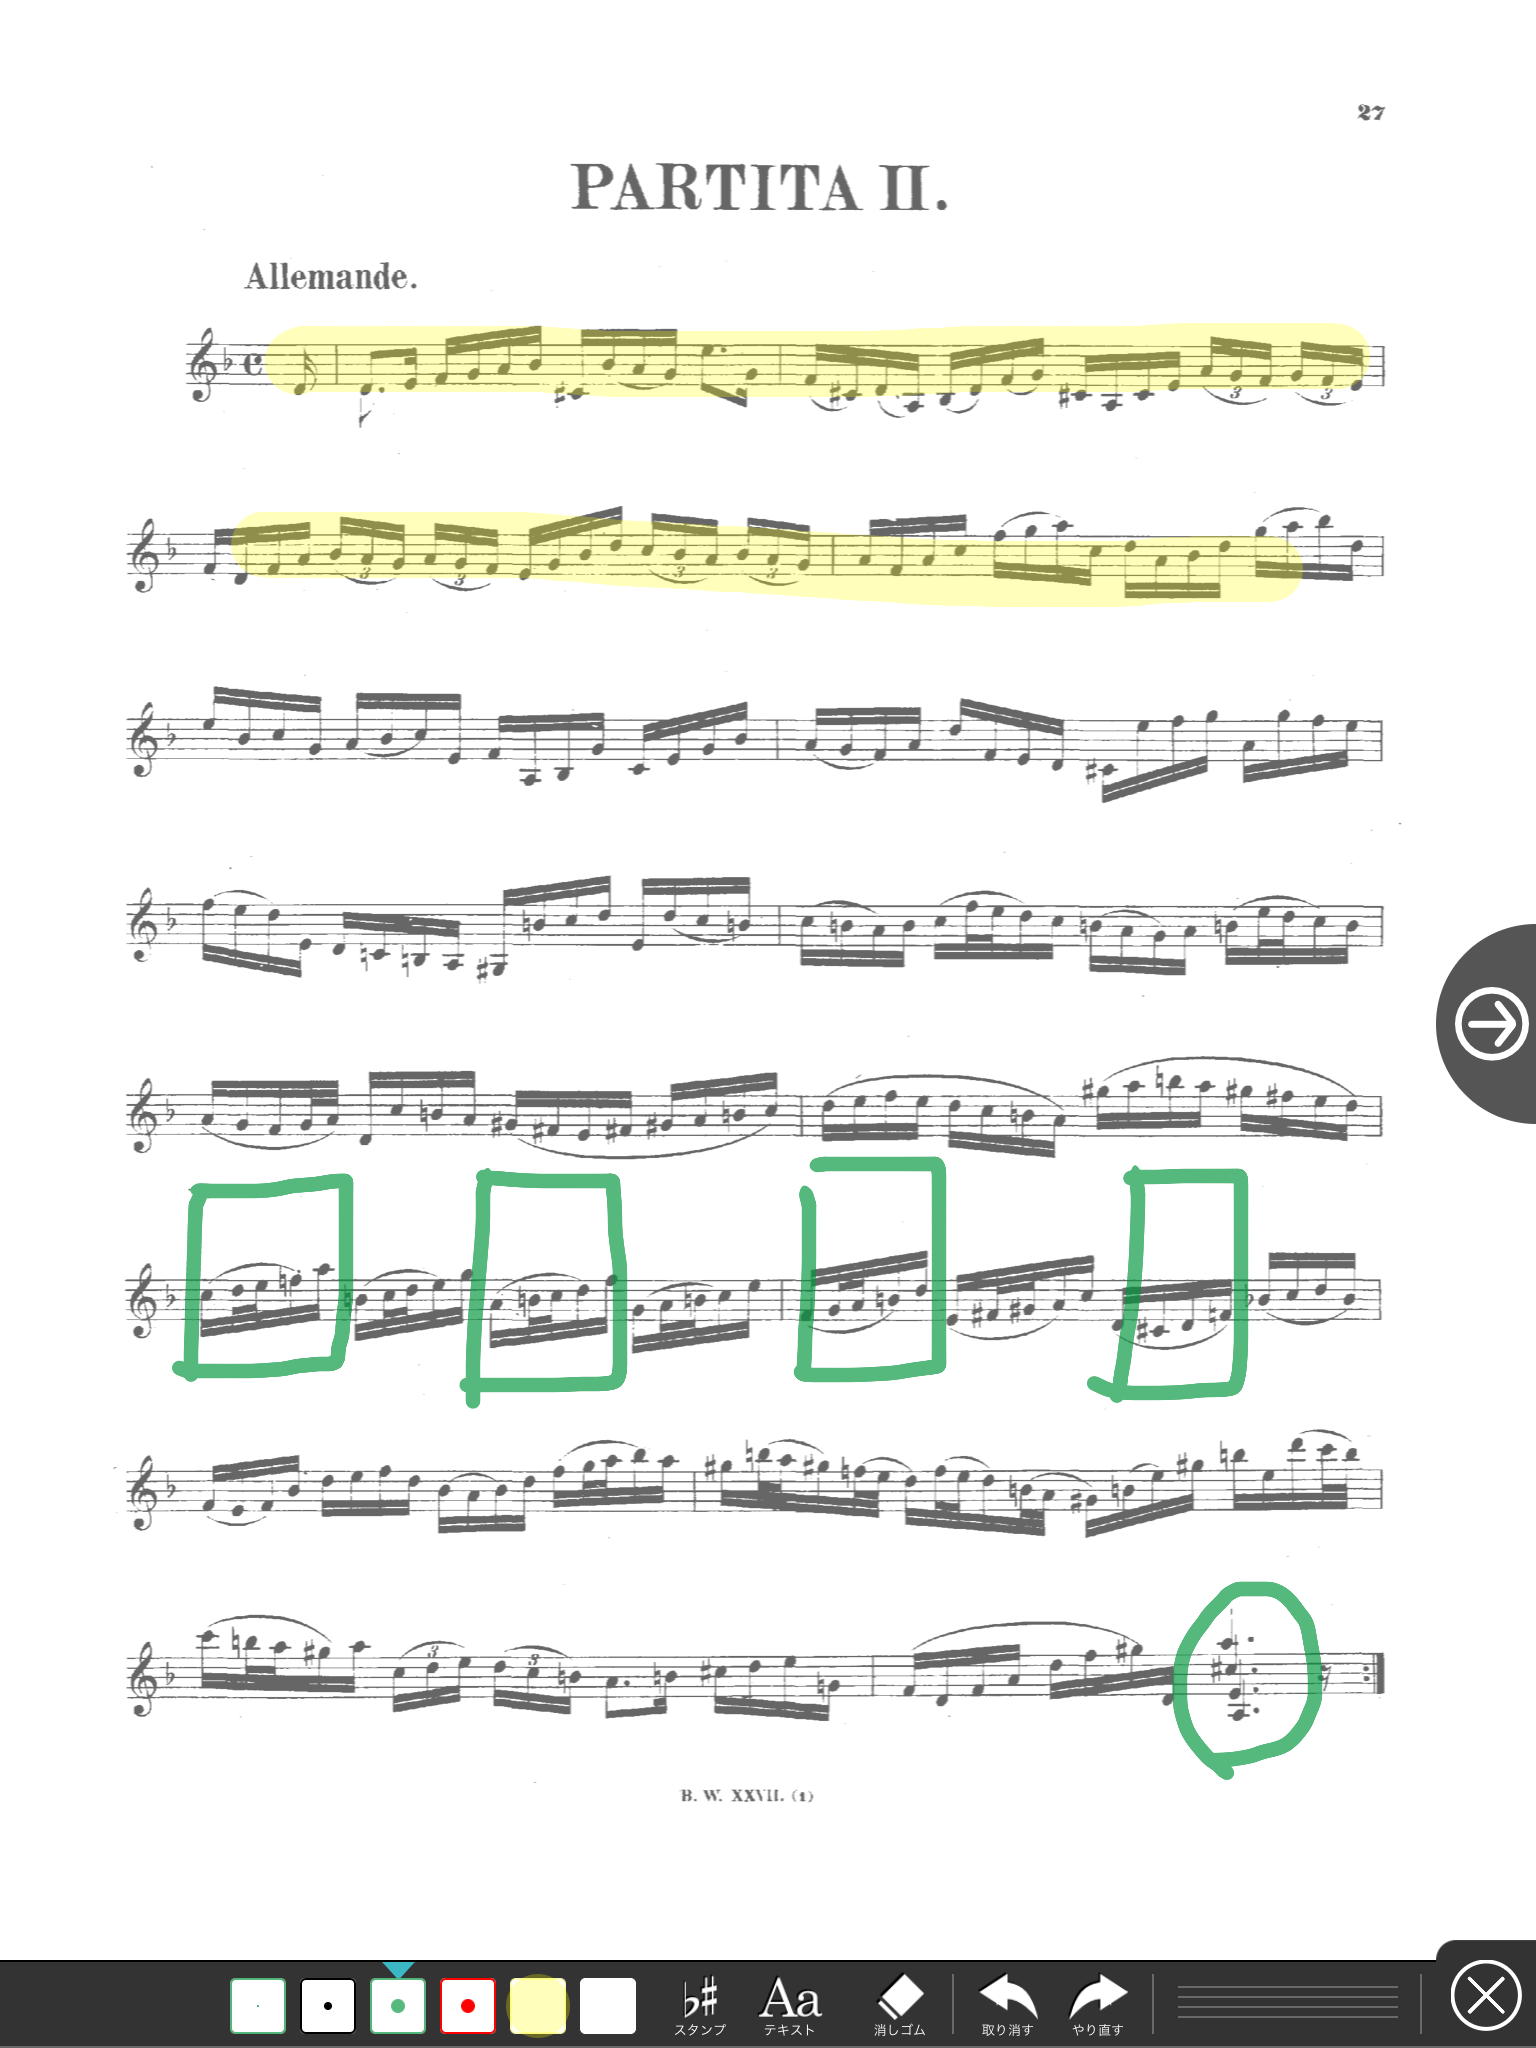
\includegraphics[width=8cm]{images/piascore.png}}
    \caption{Piascoreの画面}
    \label{pia}
\end{figure}

\section{まとめ}
楽譜の編集や閲覧を支援するシステムが広く利用されているが、これらは計算機上で楽譜の利用形態を再現したに過ぎず、
\begin{enumerate}
    \item 簡単に編集できない
    \item メモなどの情報を自在に書けない
    \item 参照や管理が面倒
\end{enumerate}という本質的な楽譜の問題は解決されていない。
次章では上記のような楽譜が持つ問題点を解決し、これまでの楽譜の在り方にとらわれない次世代の楽譜システム「ハイパー楽譜システム」を提案する。
  % 本文2
\chapter{設計}
\label{chap:sekkei}

本章ではハイパー楽譜システムの要件と設計について述べる。

\newpage

\section{要件}
前章で整理した楽譜の問題点を踏まえた上で、ハイパー楽譜システムの要件を整理する。
\begin{enumerate}
    \item 楽譜を簡単に編集できる\\
    メモを取るような気軽さで楽譜を書くことができ、新規作成/既存楽譜の編集両方を簡単に行える。
    \item メモなどの情報を自在に書ける\\
    テキストで楽譜を記述でき、ハイパーテキストのようなフォーマットの中で楽譜以外の情報も一緒に管理できる。
    \item ハイパーリンクを利用できる\\
    楽譜上の要素やテキストに対してハイパーリンクを設定でき、関連情報に素早くアクセスできる。
\end{enumerate}
この要件を満たす楽譜システムは、ハイパーテキストの編集環境であるWikiと、テキストベースの楽譜記述言語の組み合わせによって実現できる。

\section{ハイパー楽譜システム}
本研究で提案するハイパー楽譜システムの基本構成と使い方を解説する。

\subsection{基本構成}
ハイパー楽譜システム(図\ref{hs})はWikiであるScrapbox\footnote{\textsf{https://scrapbox.io}}と、楽譜記述言語のABC記譜法\footnote{\textsf{http://abcnotation.com}}(以下ABC)によって構成されている。

\begin{figure}[H]
    \centering
    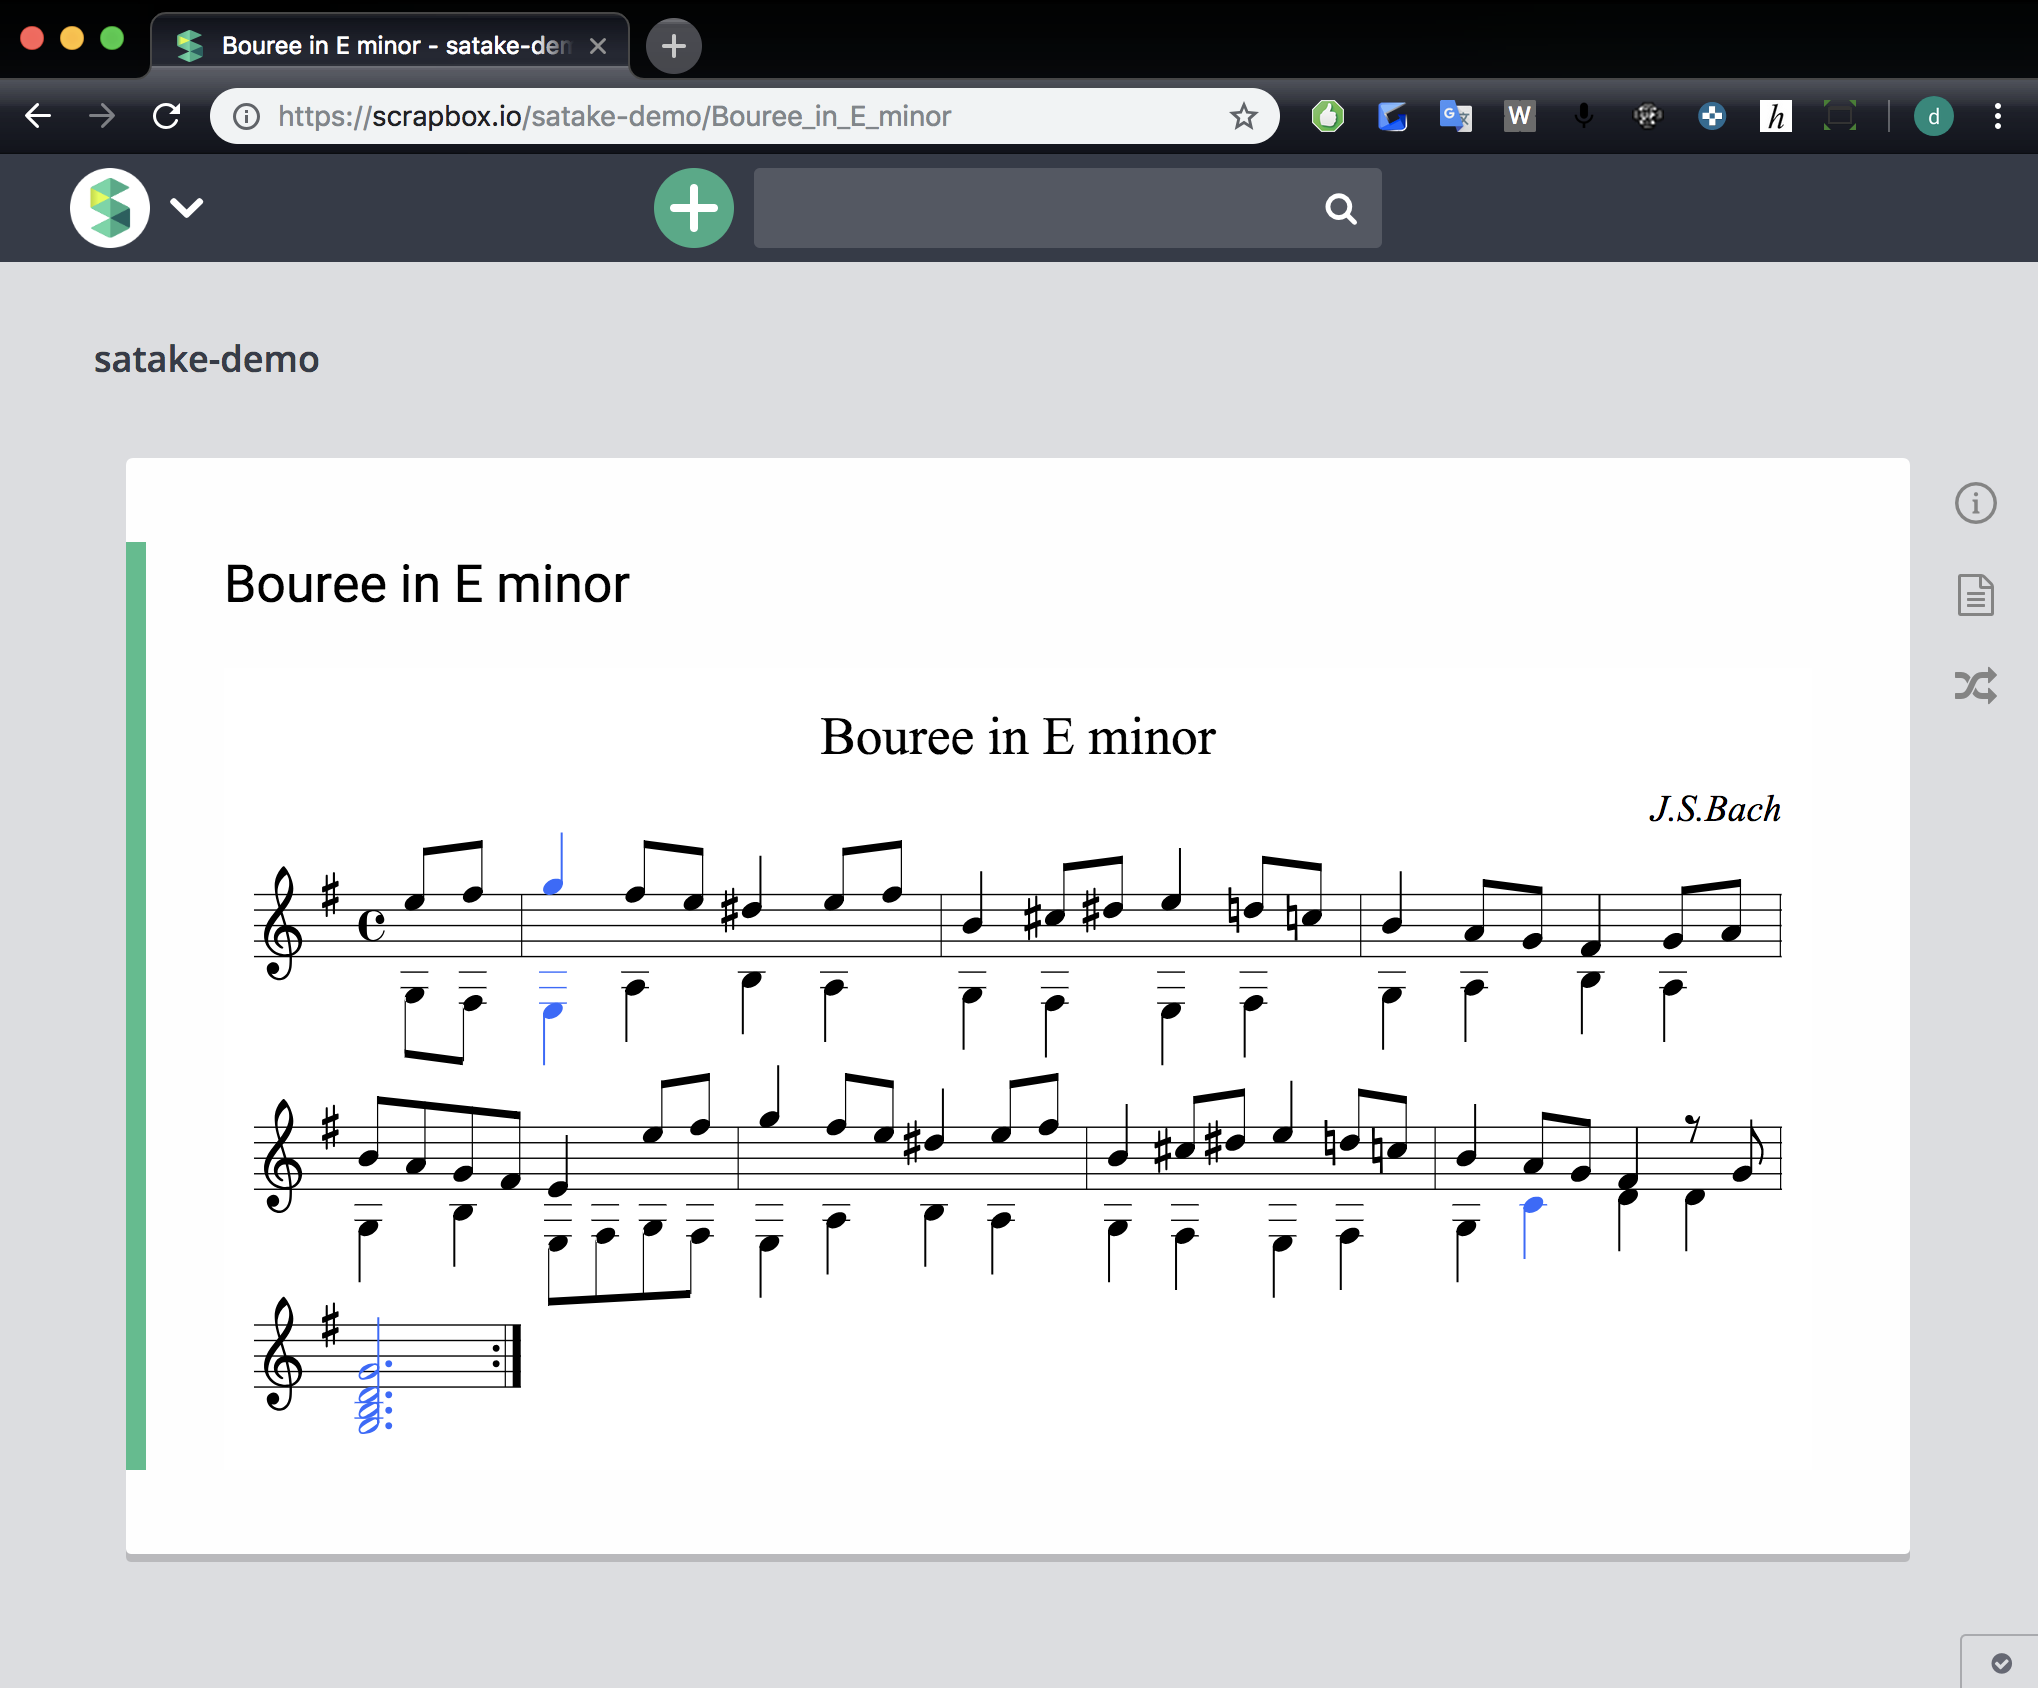
\includegraphics[width=10cm]{images/hyperscore.png}
    \caption{ハイパー楽譜システム上で書かれた楽譜}
    \label{hs}
\end{figure}


\paragraph*{Scrapbox}
Scrapbox(図\ref{scrap})はGyazz\cite{Gyazz}をベースにして開発された、Nota\footnote{\textsf{https://www.notainc.com/ja}}社が運営しているWikiである。
他のシステムには存在しない、ハイパー楽譜システムとして利用するのに最適な特徴を持つ。

\begin{itemize}
    \item シンプルで柔軟な記法をもつWYSIWYGエディタ

    入力/改行/段落/箇条書きといった基本的なテキスト編集を見たまま行える。
    またリンクやマルチメディアの埋め込みには\texttt{[]}記法のみで対応でき、他に様々な記法を覚える必要がない。

    \begin{itembox}[l]{\texttt{[]}記法}
        \begin{tabbing}
            ********************************* \= ********************** \kill
            \texttt{[ページ名]} \> 同一Wiki内ページへのリンク\\
            \texttt{[URL]} \> 外部リンク\\
            \texttt{[画像URL]} \> 画像埋め込み\\
            \texttt{[音声URL]} \> 音声埋め込み\\
            \texttt{[YouTube/VimeoURL]} \> 動画埋め込み\\
            \texttt{[GoogleMapsURL]} \> 地図埋め込み
        \end{tabbing}
    \end{itembox}

    \item 関連ページリスト

    Scrapboxページの下部には
    \begin{itemize}
        \item 別ページへのリンク
        \item 別ページからのリンク
        \item リンク先ページがリンクしているページ
    \end{itemize}といった関連ページリスト(図\ref{related})が表示され、どのような情報と関連するのか一目瞭然に分かる。

    \item リアルタイム共同編集

    Scrapboxでは複数人による共同編集だけでなく、Googleドキュメント\footnote{\textsf{https://www.google.com/intl/ja\_jp/docs/about}}のようなリアルタイム編集作業をコンフリクトすることなく行うことが可能である。
\end{itemize}

\begin{figure}[H]
    \centering
    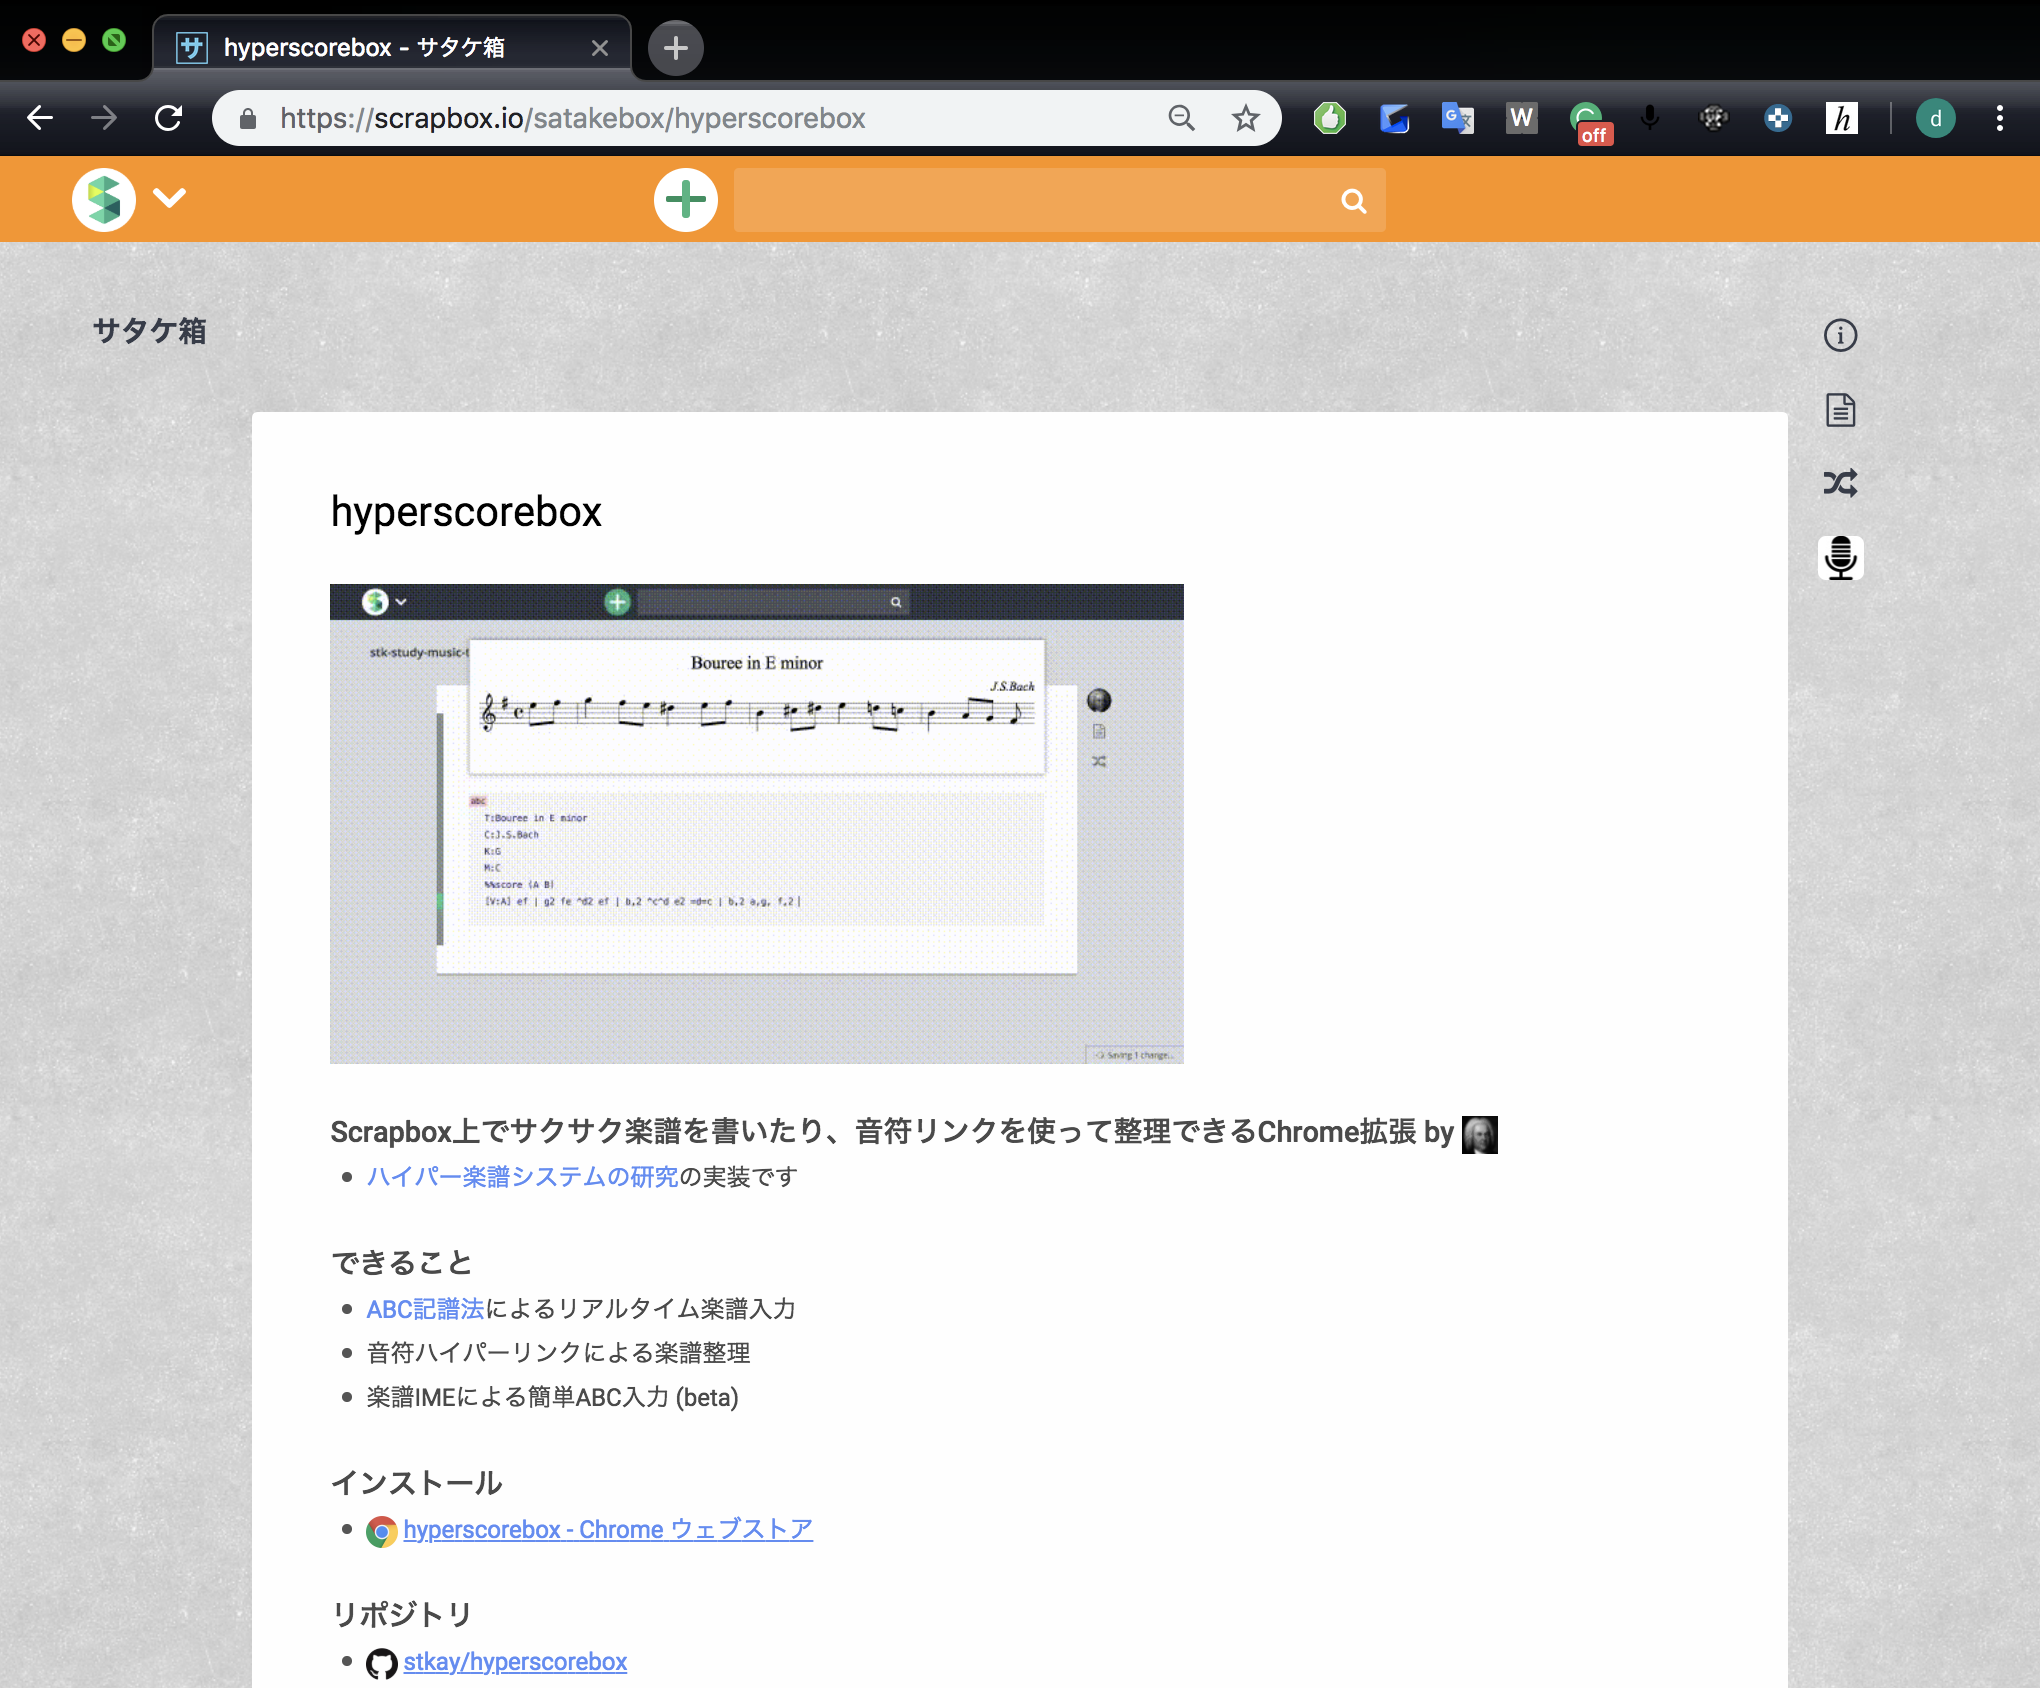
\includegraphics[width=10cm]{images/scrapbox.png}
    \caption{Scrapboxの画面}
    \label{scrap}
\end{figure}

\begin{figure}[H]
    \centering
    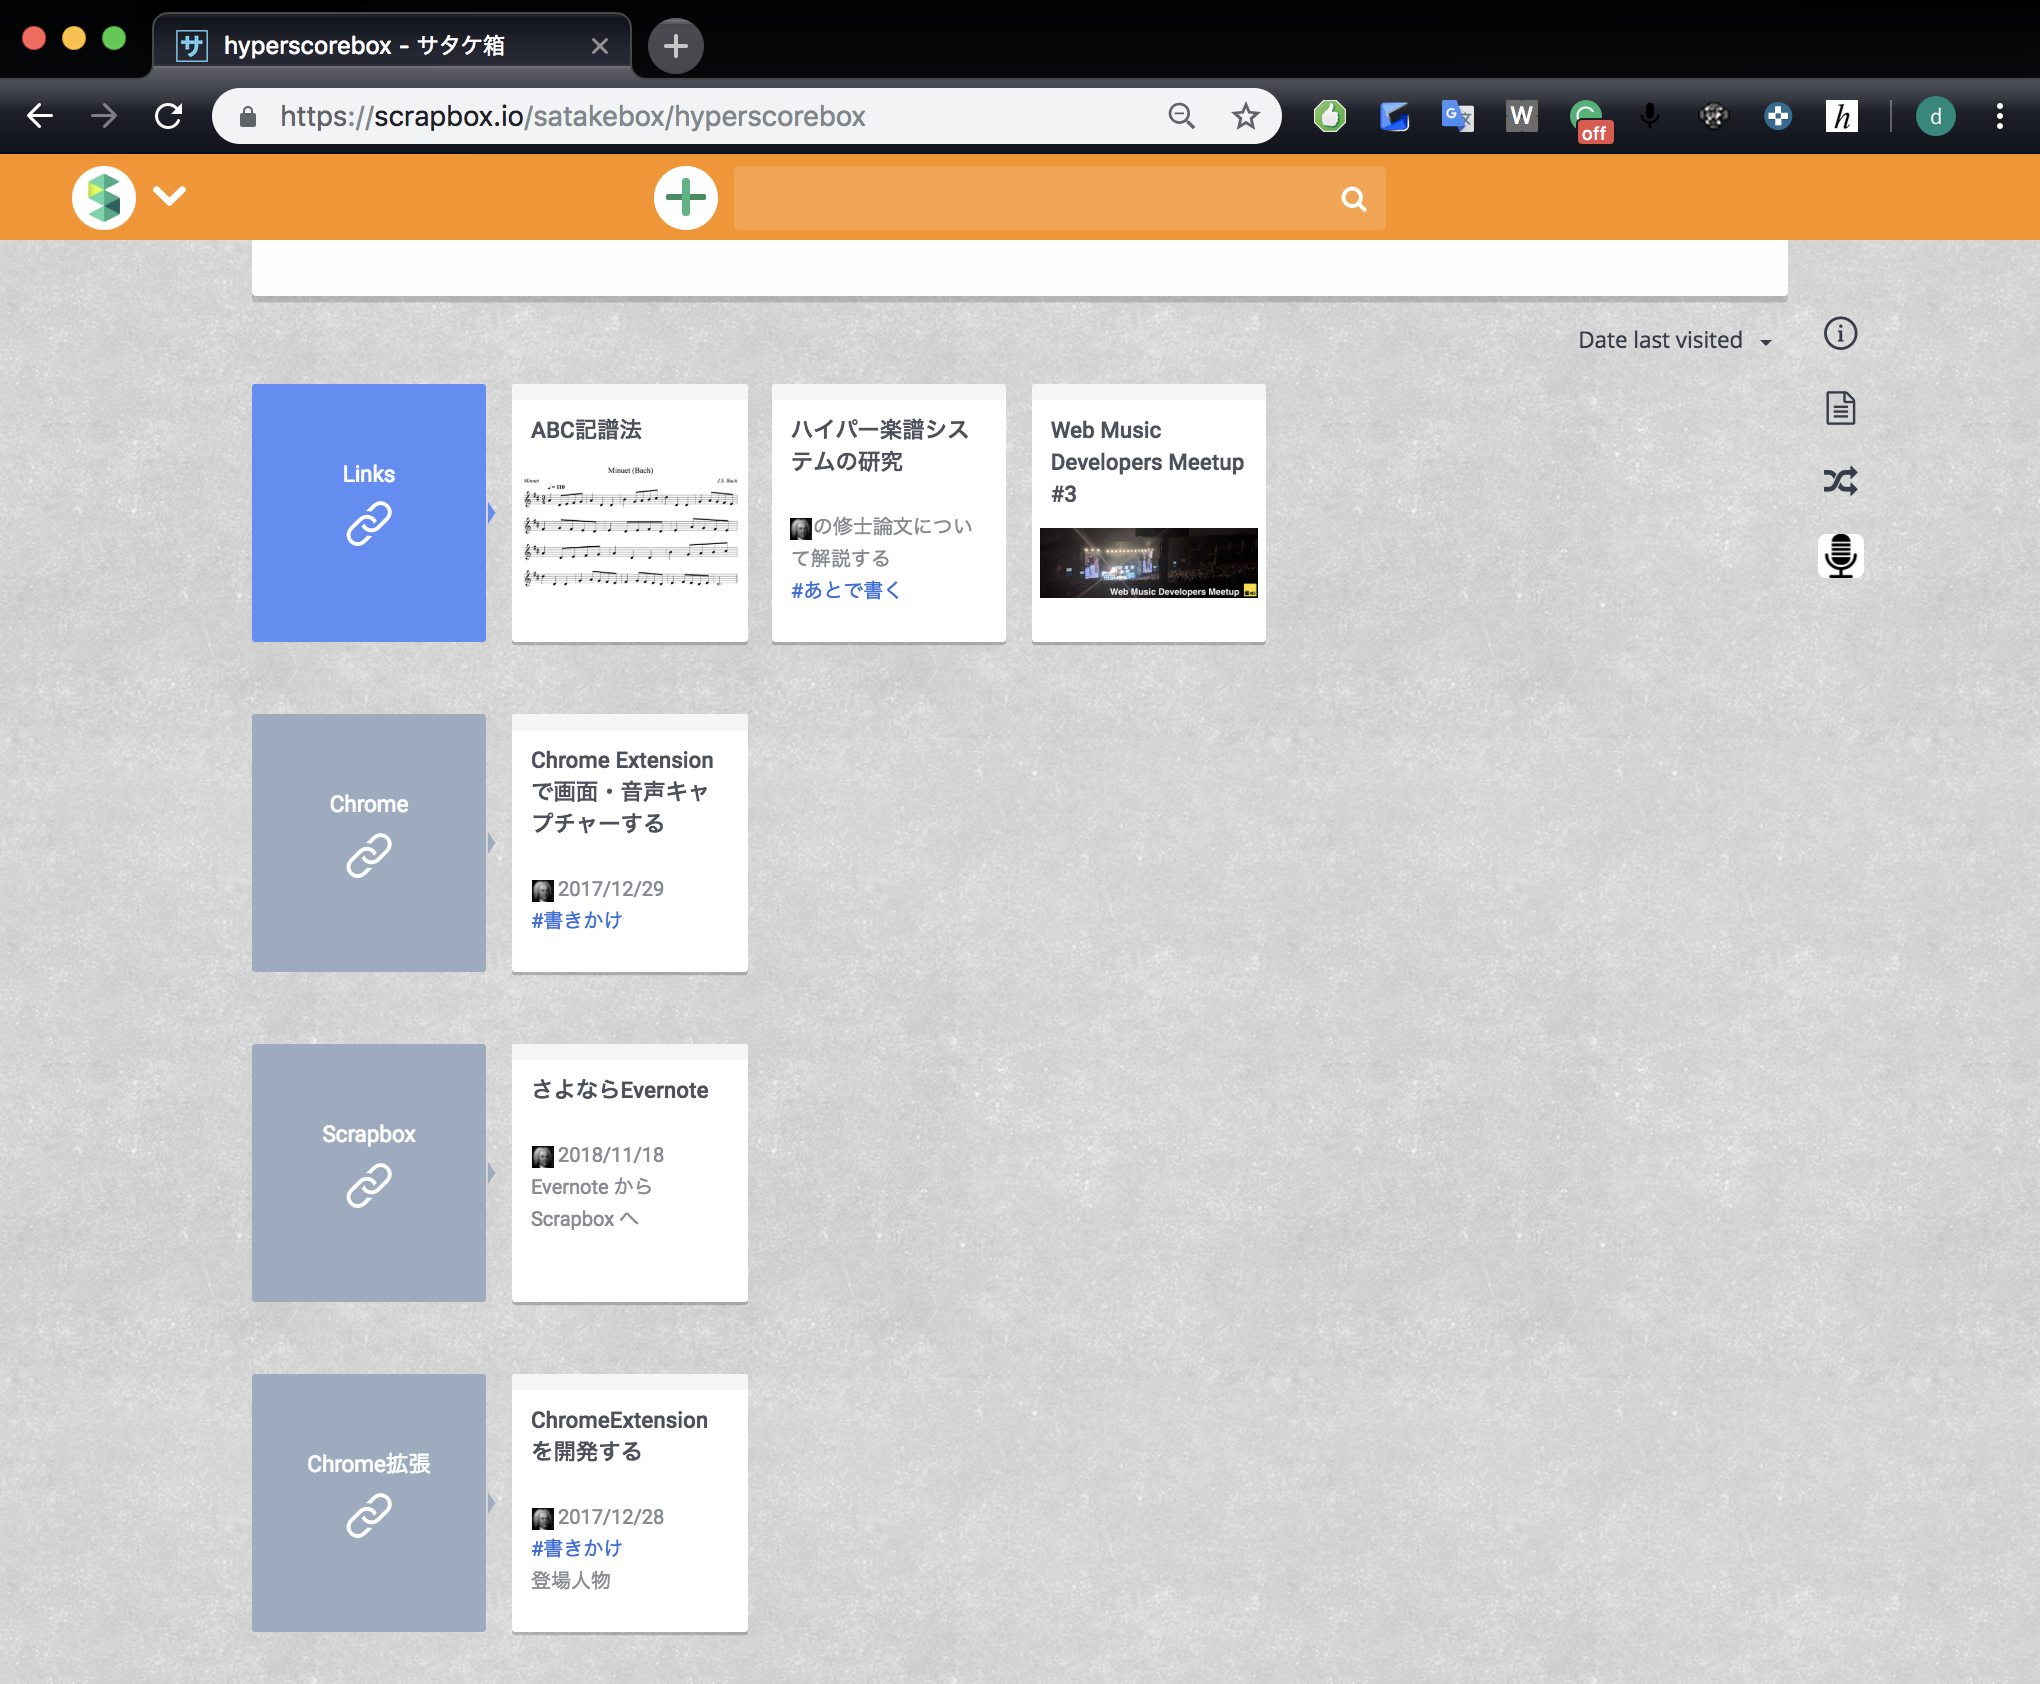
\includegraphics[width=10cm]{images/related.png}
    \caption{関連ページリスト}
    \label{related}
\end{figure}

\paragraph*{ABC}
ABCはプレーンテキスト形式の楽譜記述言語で、\texttt{c}が「ド」を表すシンプルな記法(ソースコード\ref{abctext})を持つ。
大規模で複雑な楽譜(図\ref{complex})の記述も可能で、幅広いシーンで利用可能である。
利用者コミュニティ\footnote{\textsf{https://groups.yahoo.com/neo/groups/abcusers/info}}が活発でバージョンのアップデートが頻繁に行われていたり、ユーザーによる譜例が多く公開されていることから信頼できるフォーマットである。
ブラウザからはJavaScriptライブラリのabcjs\footnote{\textsf{https://abcjs.net/}}が利用でき、既存の楽譜システムと比較しても遜色のない綺麗な楽譜を出力することが可能である。

\begin{lstlisting}[caption=「ド」を表すABC, label=abctext]
    c
\end{lstlisting}
\begin{figure}[H]
\centering
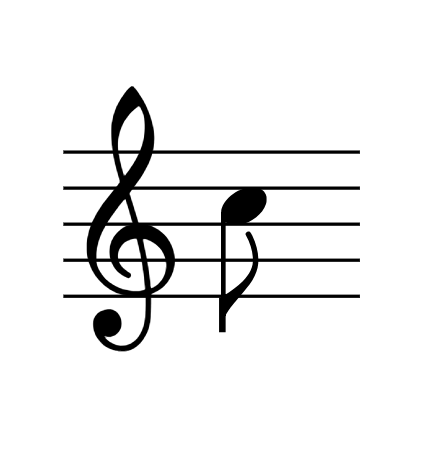
\includegraphics[width=2cm]{images/c.png}
\caption{「ド」の譜例}
\label{abcnote}
\end{figure}

\begin{figure}[H]
\centering
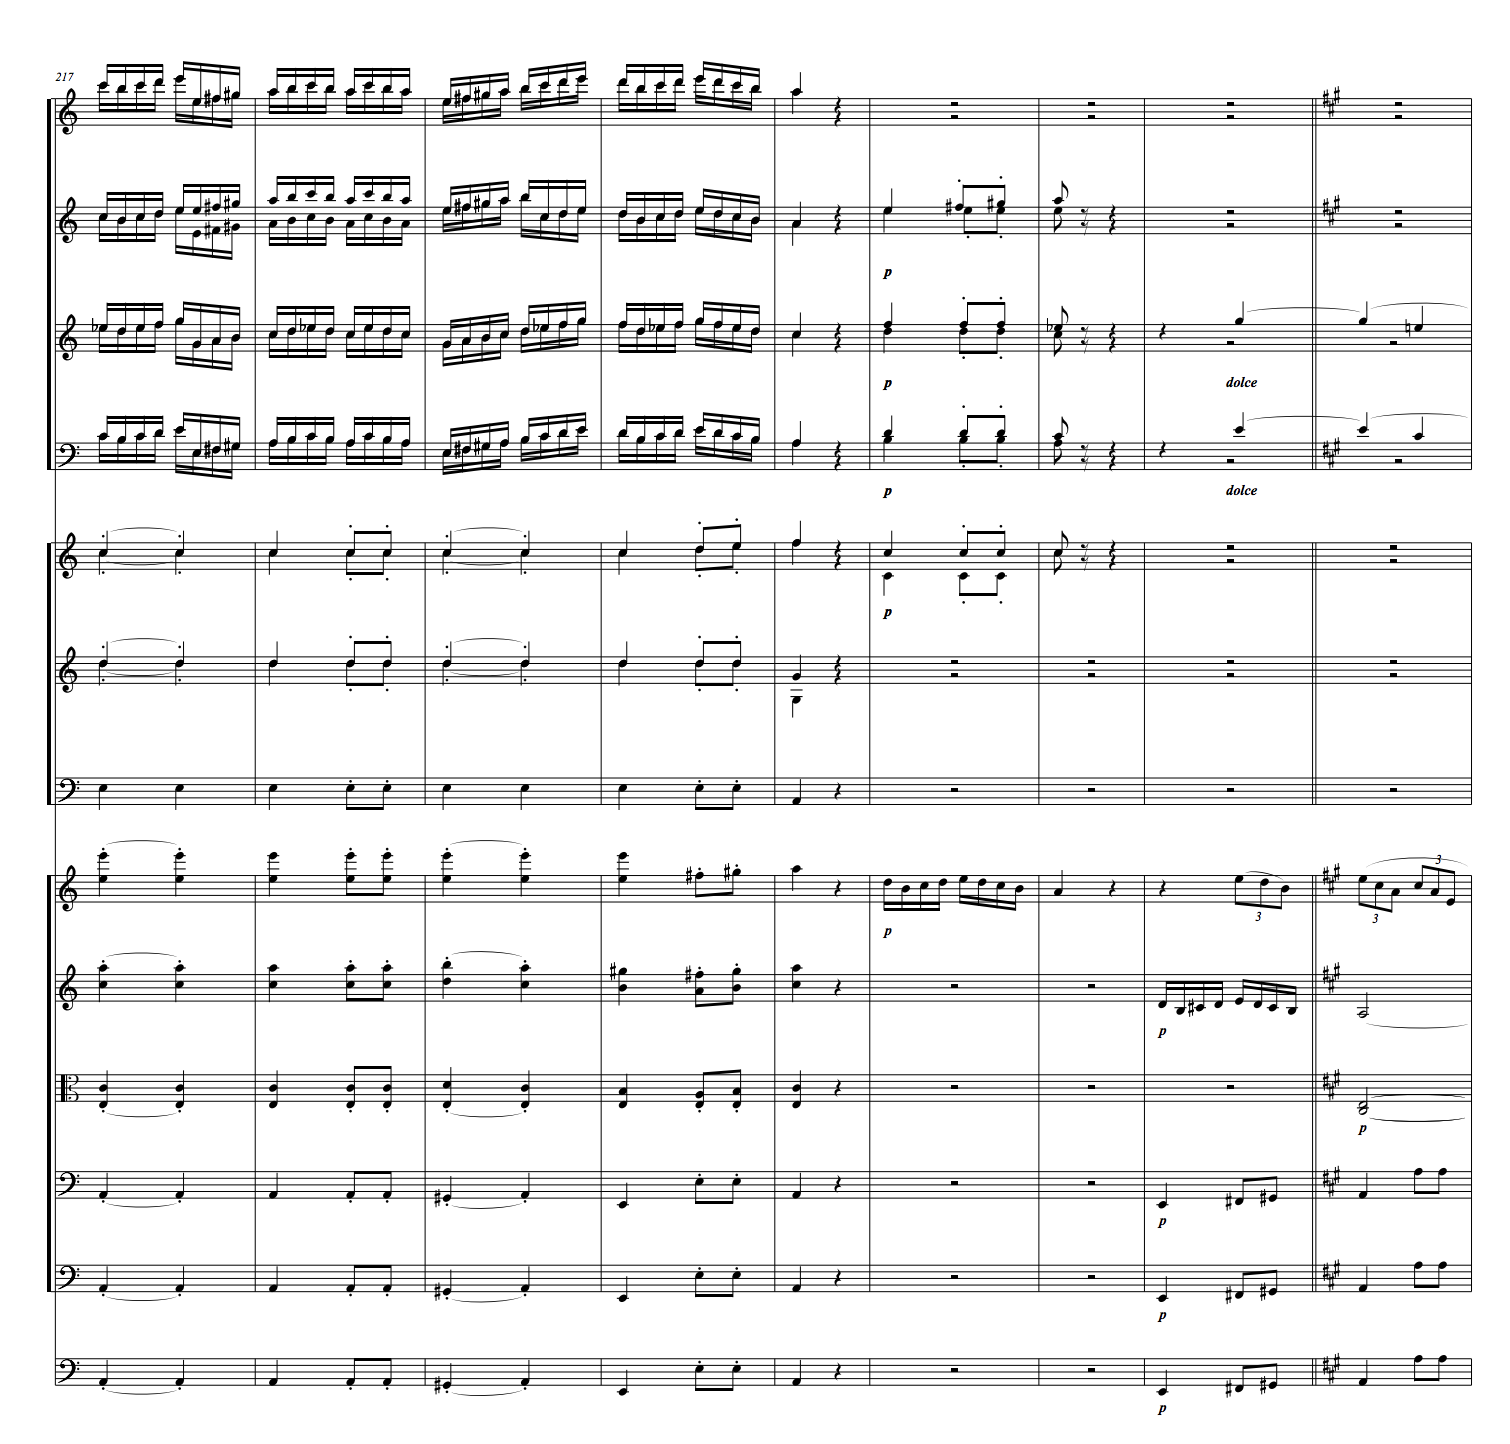
\includegraphics[width=10cm]{images/complexabc.png}
\caption{複雑な楽譜の例}
\label{complex}
\end{figure}


\subsection{使い方}
\paragraph*{楽譜を書く}
Scrapbox上で\texttt{code:*.abc}という行に続けてABCテキストを書くとABC記述の真上に楽譜画像が表示され(図\ref{editingabc})、楽譜を確認しながらリアルタイムに編集できる。
楽譜やABCの領域外をクリックするとABC記述が隠れ、楽譜のみが表示される(図\ref{editedabc})。

\begin{figure}[H]
\centering
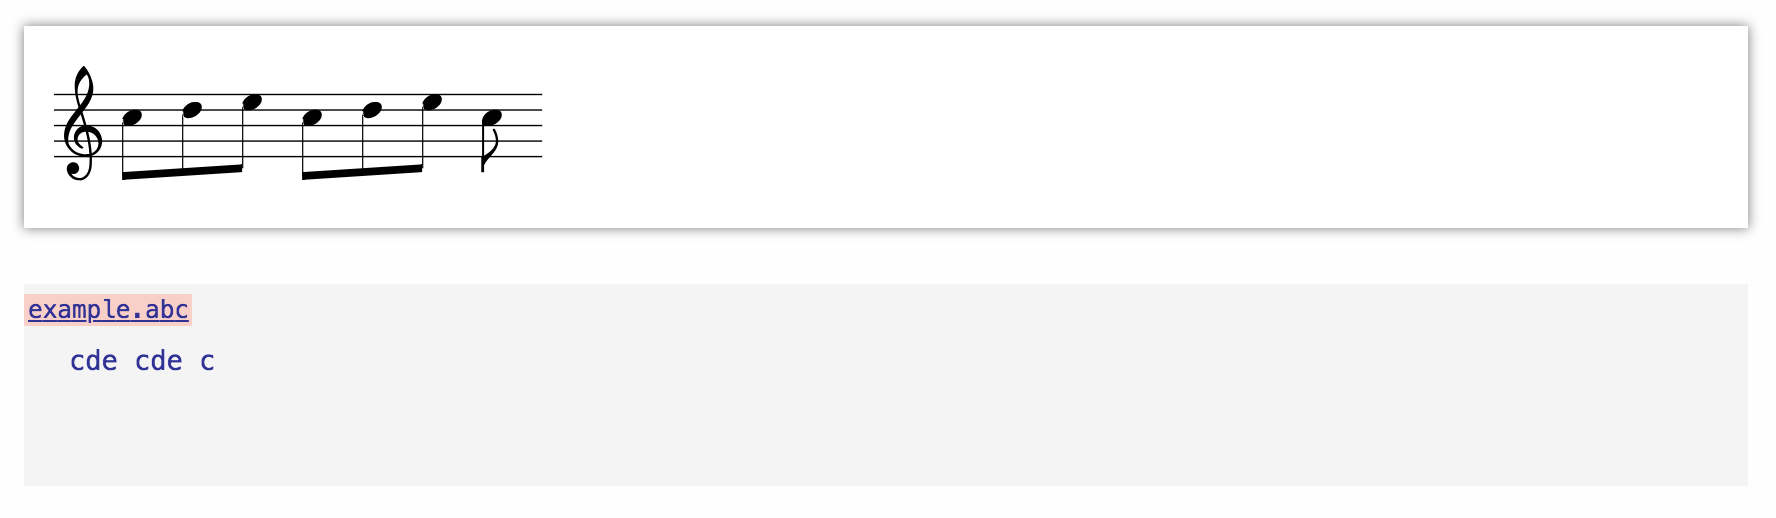
\includegraphics[width=10cm]{images/editingabc.png}
\caption{編集中の楽譜}
\label{editingabc}
\end{figure}

\begin{figure}[H]
\centering
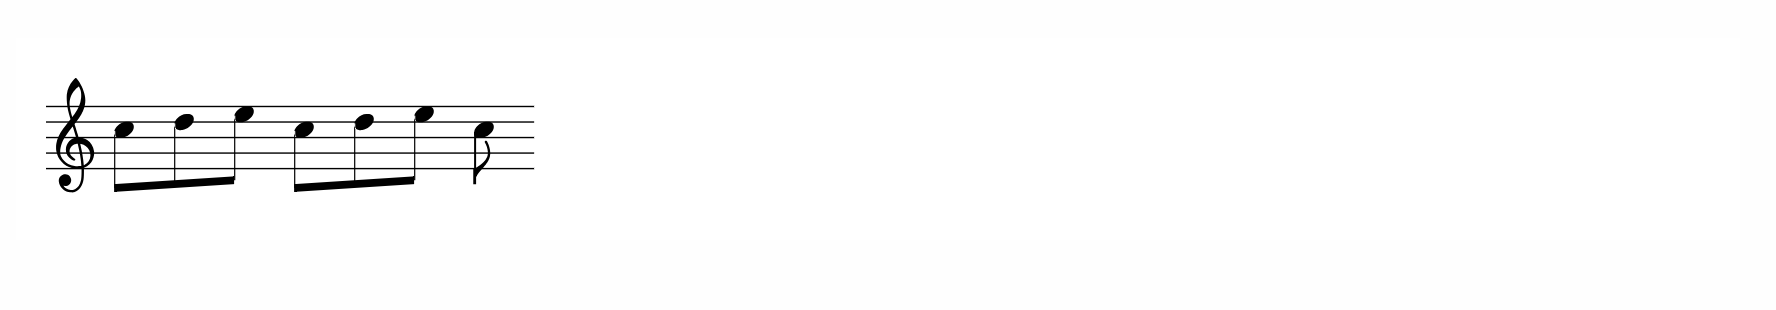
\includegraphics[width=10cm]{images/editedabc.png}
\caption{編集後の楽譜}
\label{editedabc}
\end{figure}


\paragraph*{音符など以外の情報を書く}
楽譜領域以外では標準のScrapbox記法を利用できるので、自在にテキストを書いたり、マルチメディアを埋め込むことができる(図\ref{scoreandtext})。

\begin{figure}[H]
\centering
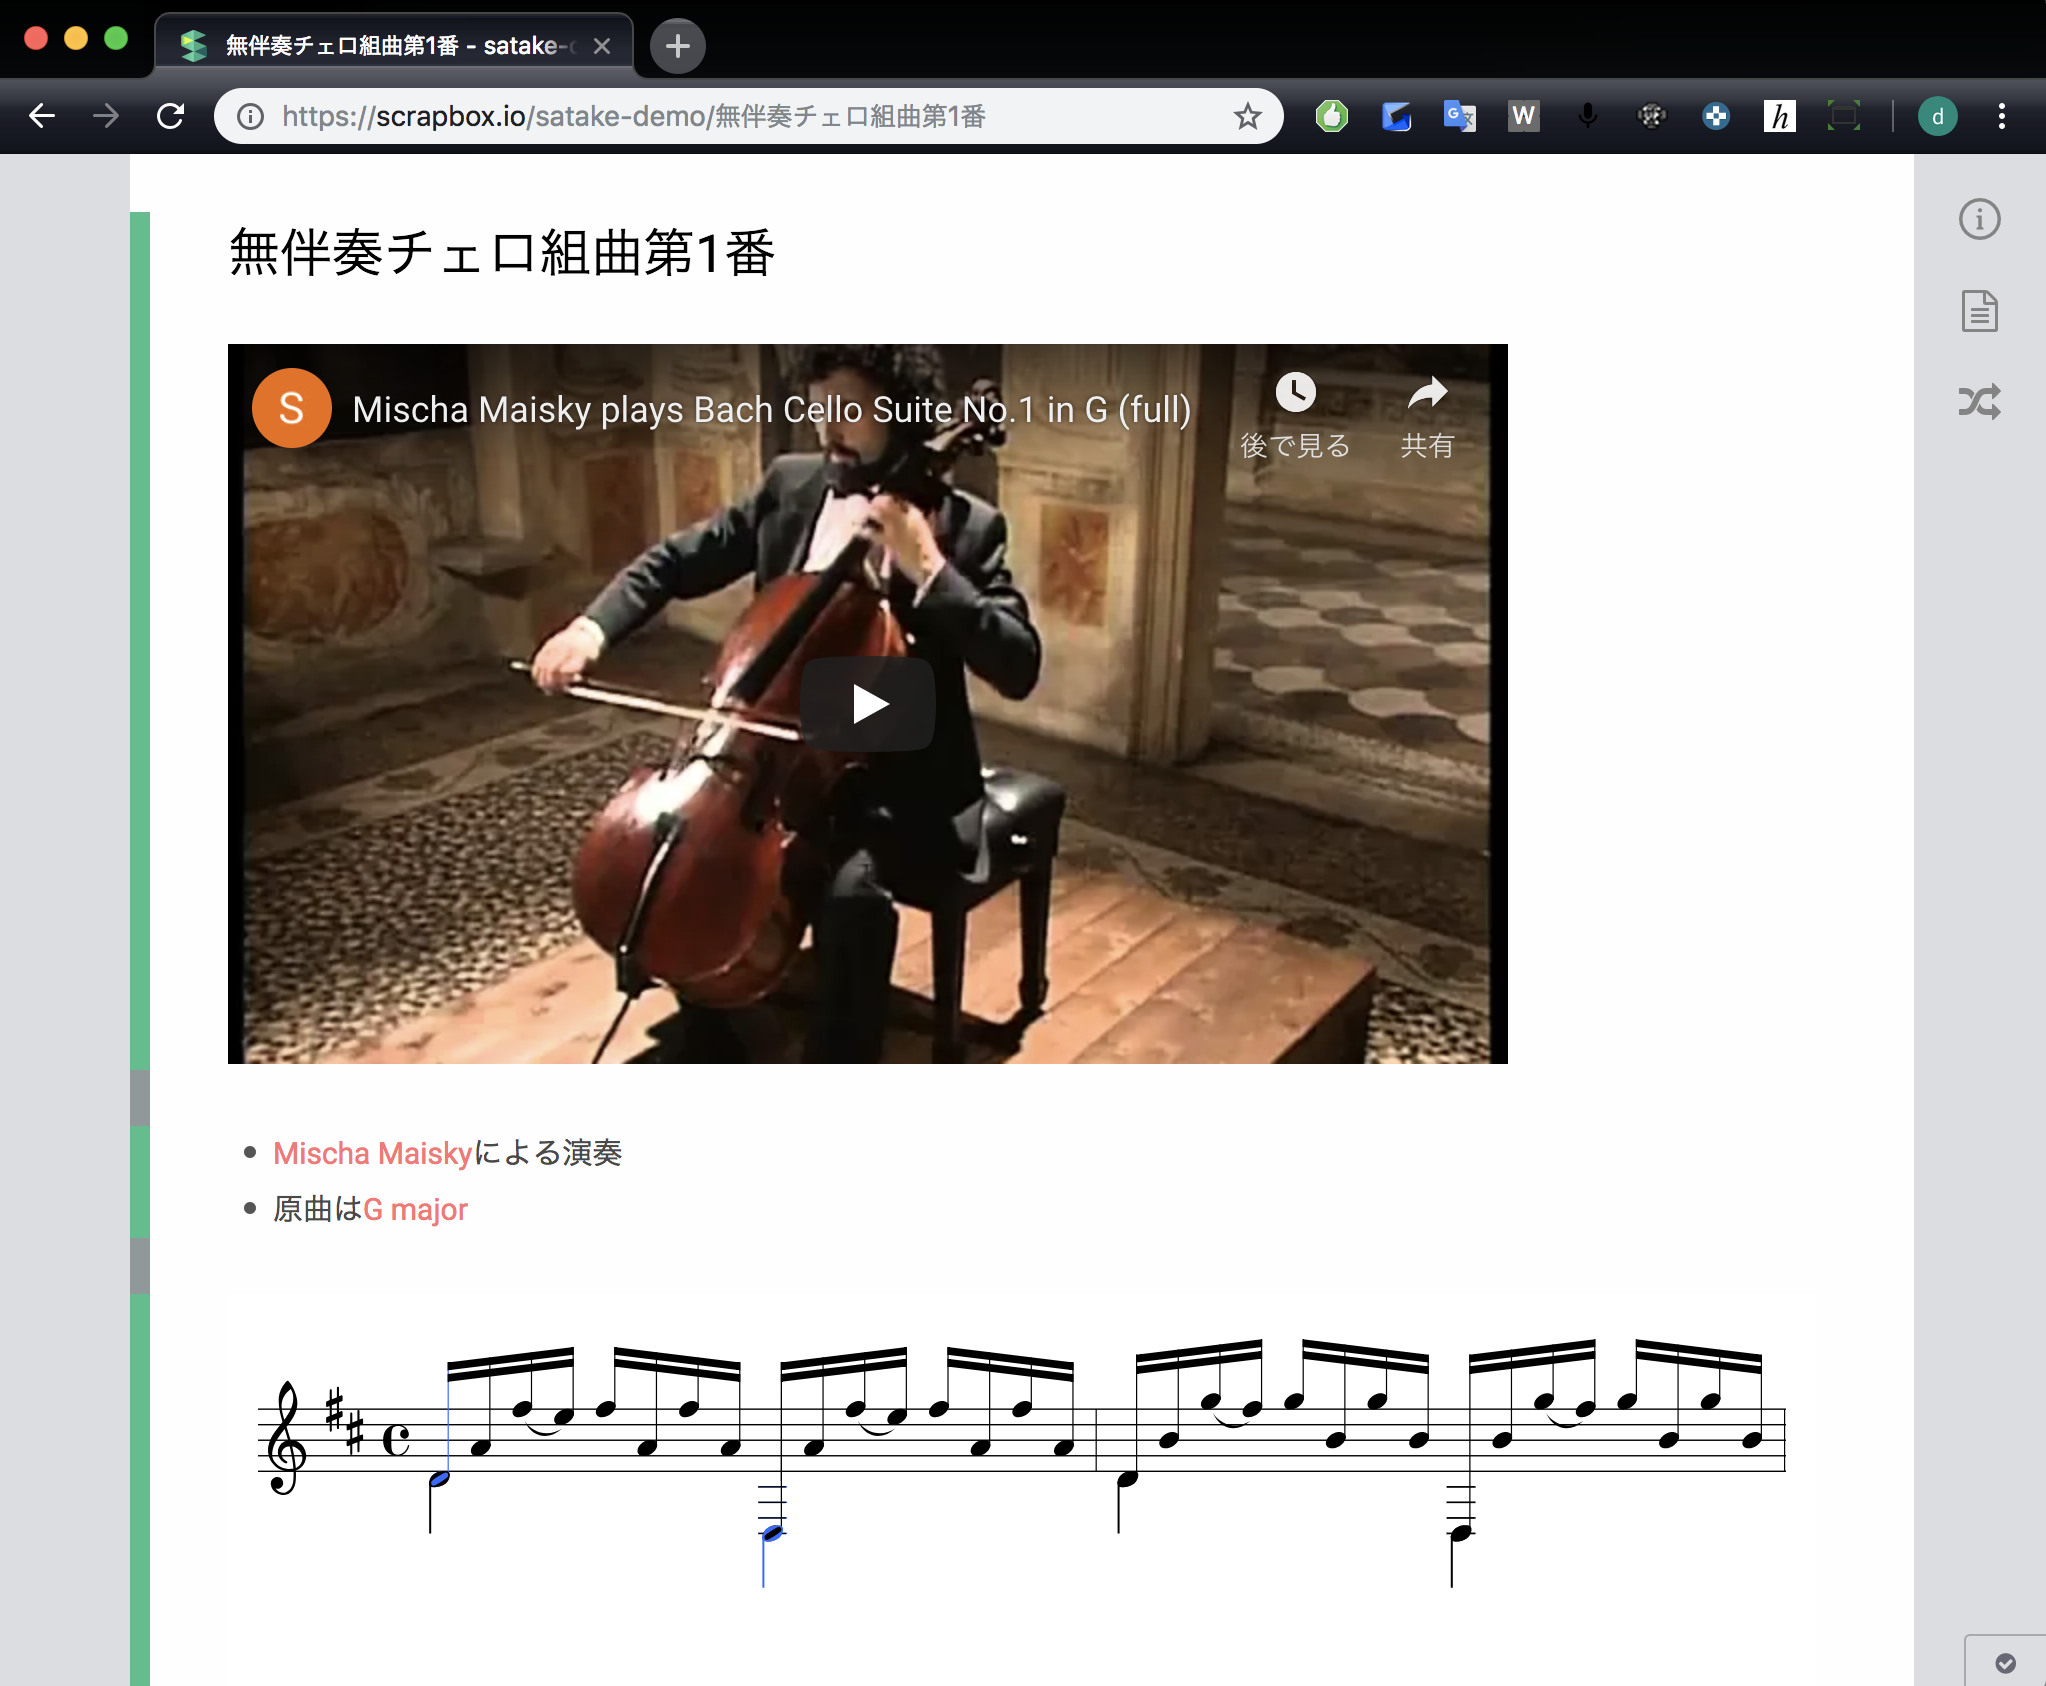
\includegraphics[width=10cm]{images/scoreandtext.png}
\caption{楽譜にテキストや動画が埋め込まれた例}
\label{scoreandtext}
\end{figure}


\paragraph*{ハイパーリンクを利用する}
ABCには無い独自の機能として音符ハイパーリンク機能を利用できる。
ABCの末尾に\texttt{\%Links:[リンク1][リンク2]…}と記述することで対象となる音符にハイパーリンクを設定できる。
具体的な設定方法とその例を図\ref{linkabc}に示す。
ハイパーリンクが設定された音符は青く表示され(図\ref{linkednote})、クリックするとリンク先のページへ遷移する(図\ref{middlec})。

\begin{figure}[H]
\centering
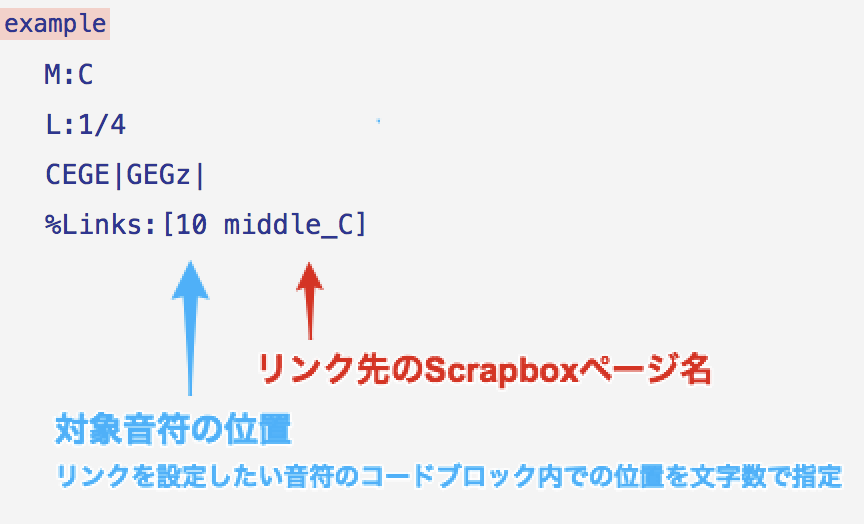
\includegraphics[width=10cm]{images/linkabc.png}
\caption{1音目の「C」に「middle C」ページへのリンクが設定されたABC}
\label{linkabc}
\end{figure}

\begin{figure}[H]
\centering
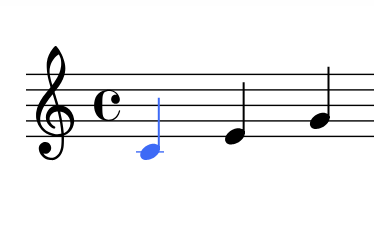
\includegraphics[width=4cm]{images/linkednote.png}
\caption{ハイパーリンクが設定された音符}
\label{linkednote}
\end{figure}

\begin{figure}[H]
\centering
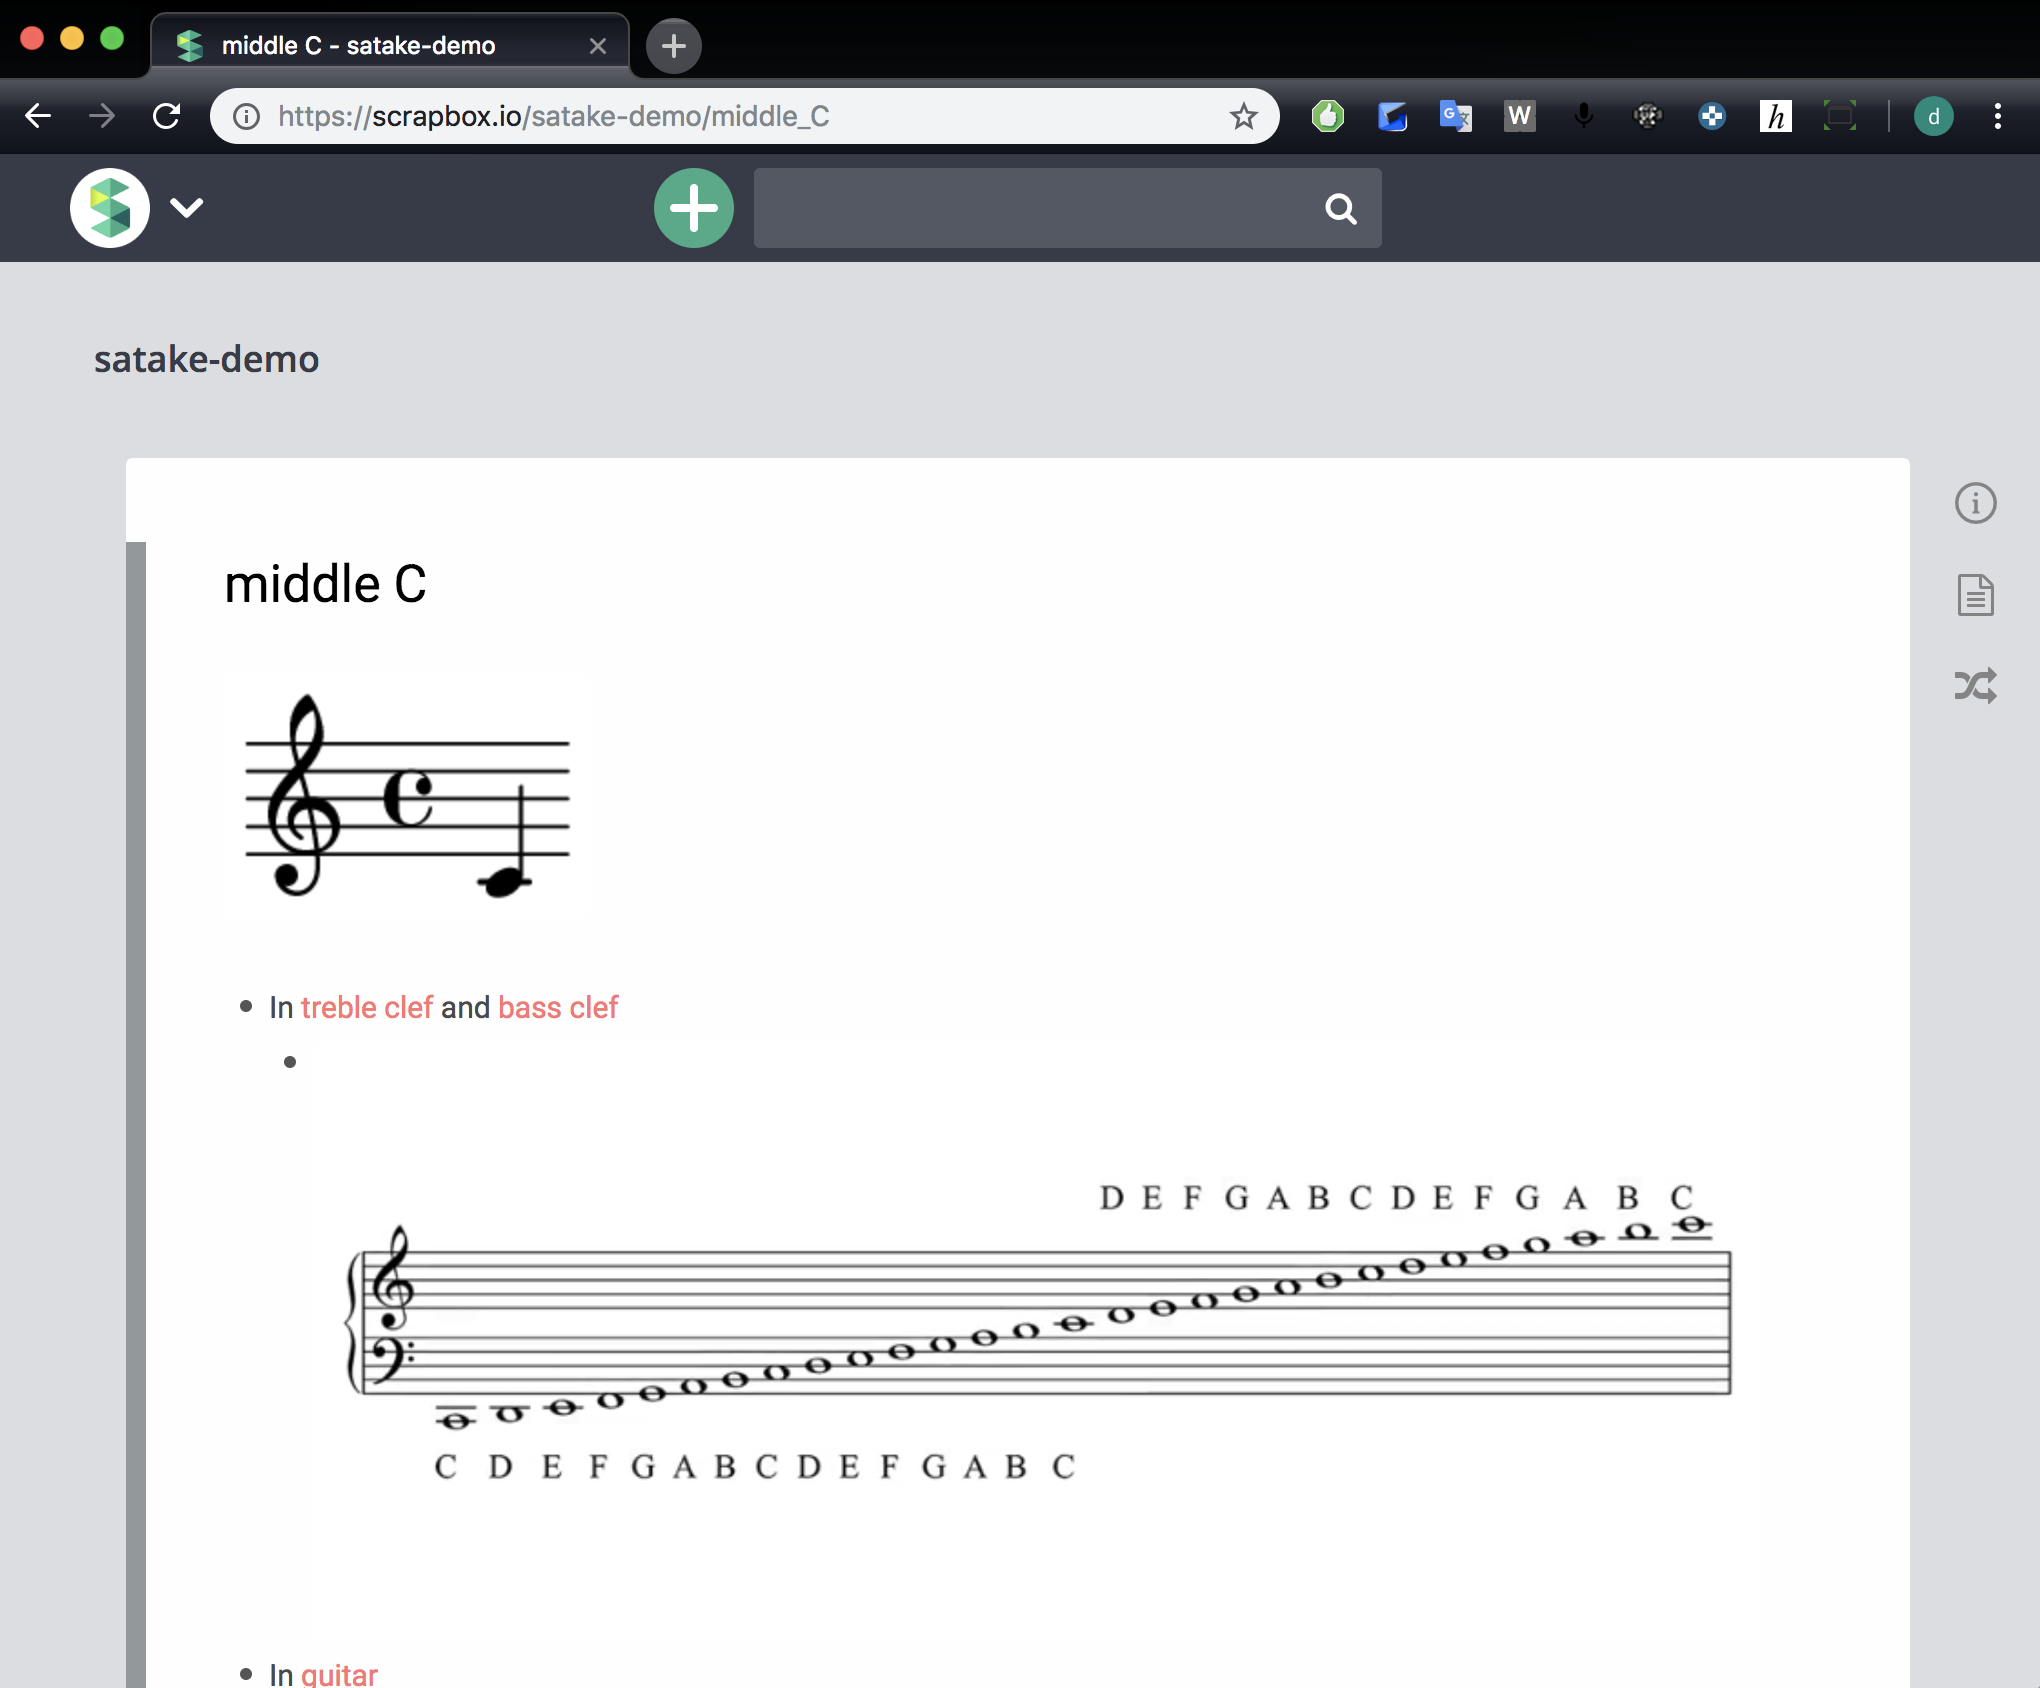
\includegraphics[width=10cm]{images/middlec.png}
\caption{リンク先の「middle C」ページ}
\label{middlec}
\end{figure}

  % 本文3
\chapter{実装}
\label{chap:jissou}

本章では第\ref{chap:sekkei}章で述べたシステムの設計を受け、ハイパー楽譜システムの実装について述べる。

\newpage

\section{アプリケーション構成}
ハイパー楽譜システムはScrapbox上で利用するChrome Extensionとして実装されている\footnote{\textsf{https://chrome.google.com/webstore/detail/hyperscorebox/cjlhoobllhkpjjomlijlfdblgifcdmoh}}。
Chrome Extensionをインストール可能なPC版Google Chromeを利用できる環境であれば、OSを問わず利用することができる。
Chrome Extensionの開発にはTypeScript\footnote{\textsf{https://www.typescriptlang.org/}}を、楽譜の出力にはabcjsを利用している。
%以下に本システムの構成図を示す。
%イラストでも書く

\paragraph*{Chrome Extension}
Chrome ExtensionはGoogle Chrome上にインストール可能なブラウザの機能を拡張できるアプリケーションである。
一般的なWebページと同様に、HTML/CSS/JavaScriptのようなWeb技術を用いて実装することができ、
\begin{itemize}
    \item HTML要素の操作
    \item カスタムCSSの適用
    \item HTTPリクエスト
    \item 外部サービスとの連携
\end{itemize}といった機能が実現可能である。
アプリケーションはChrome Web Store\footnote{\textsf{https://chrome.google.com/webstore/category/extensions?hl=ja}}を通じて簡単に公開できる。

\section{楽譜の描画}
本節では楽譜描画の仕組みを述べる。

Scrapboxにはコードハイライトを行うコードブロック記法(図\ref{codeblock})が存在し、\texttt{"code:{ファイル名}"}と入力することで利用できる。
本アプリケーションではABCの記述にこのコードブロックを利用している。
本アプリケーションによってファイル名の拡張子が\texttt{*.abc}に一致するコードブロック(図\ref{abcblock})のみがABCとして解釈され、abcjsによって生成された楽譜画像(図\ref{cde})がコードブロックのHTML要素に対して重畳表示される。

\begin{figure}[H]
    \centering
    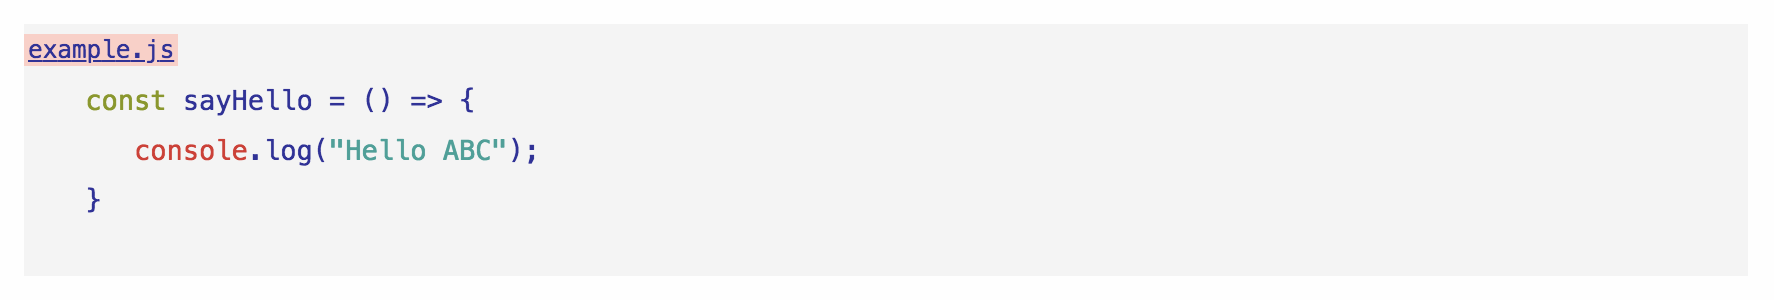
\includegraphics[width=15cm]{images/codeblock.png}
    \caption{コードブロック記法}
    \label{codeblock}
\end{figure}

\begin{figure}[H]
    \centering
    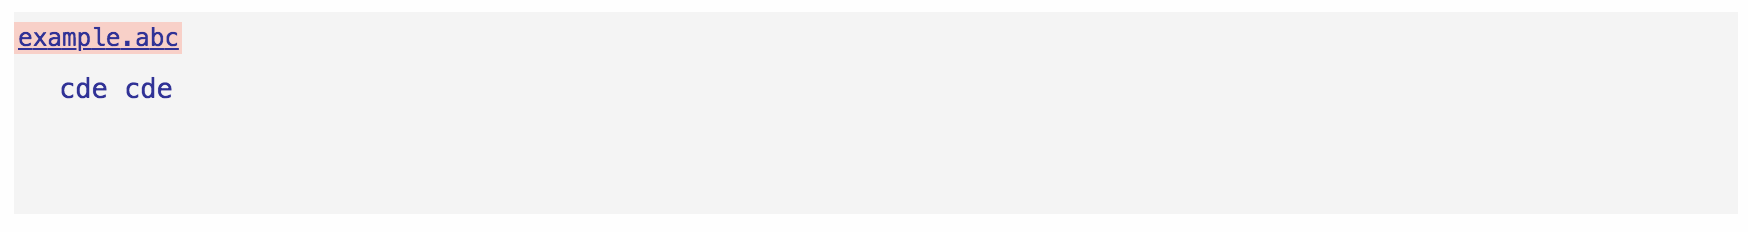
\includegraphics[width=15cm]{images/abcblock.png}
    \caption{ABCとして解釈されるコードブロック}
    \label{abcblock}
\end{figure}

\begin{figure}[H]
    \centering
    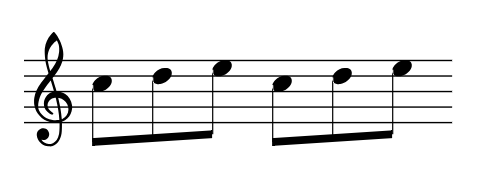
\includegraphics[width=5cm]{images/cdecde.png}
    \caption{生成された楽譜画像}
    \label{cde}
\end{figure}

\section{音符ハイパーリンク機能の実現}
本節では音符ハイパーリンク機能の実現方法を述べる。

abcjsはSVG画像として楽譜を出力しており、一つ一つの音符に対してクリックリスナを設定可能である。
\texttt{Document.location.href}オブジェクト\footnote{\textsf{https://developer.mozilla.org/ja/docs/Web/API/Location}}を利用してページ遷移を実行するコールバック関数を音符のクリックリスナに設定している。
  % 本文4

\begin{acknowledgment}

学部から5年間の長きに渡りご指導を賜りました慶應義塾大学環境情報学部 増井俊之教授に深く感謝いたします。また、本研究の副査としてご意見、ご助言を頂きました小川克彦教授、中西泰人教授に感謝いたします。

学部・修士の4年間を共に過ごし、自身の研究について幅広い議論をしていただいた政策・メディア研究科修士課程の早川匠氏、様々な形でアドバイスをくださった増井俊之研究会OB諸氏に感謝いたします。

\end{acknowledgment}
  % 謝辞。要独自コマンド、include先参照のこと

\begin{bib}[100]
\bibliography{main}
\end{bib}
  % 参考文献。要独自コマンド、include先参照のこと
\appendix
\include{92_appendix}    % 付録

\end{document}
